\documentclass[aspectratio=169,10pt]{beamer}
% Shared preamble for the talks (Beamer, Metropolis theme)
\usetheme[progressbar=frametitle,numbering=fraction,background=light,block=fill,sectionpage=none]{metropolis}
\usepackage[T1]{fontenc}
\usepackage{FiraSans}
\usepackage[scaled=.85]{FiraMono}
\usepackage{amsmath,amssymb}
\usefonttheme[onlymath]{serif}
\usepackage{booktabs,array,tabularx,multirow}
\usepackage{tikz,pgfplots}
\usepackage{fontawesome5}
\usepackage{qrcode}
\usepackage{xcolor}
\hyphenpenalty=10000\exhyphenpenalty=10000
\usepackage{ragged2e}
\usepackage{adjustbox}
\usepackage{multicol}
\newenvironment{sfig}[1][0.80]{\begin{adjustbox}{max width=\linewidth,max totalheight=#1\textheight,center}}{\end{adjustbox}}
\usetikzlibrary{arrows.meta,positioning,shapes.geometric,shapes.misc,fit,calc,backgrounds,decorations.pathreplacing,patterns,matrix,chains}
\usepgfplotslibrary{fillbetween}
\pgfplotsset{compat=1.17}

% ---- palette (matches vinhqdang.github.io) ----
\definecolor{tdInk}{HTML}{1D2330}
\definecolor{tdMuted}{HTML}{5D6678}
\definecolor{tdLine}{HTML}{D9D5CA}
\definecolor{tdPaper}{HTML}{FBFAF7}
\definecolor{tdBlue}{HTML}{2457D6}
\definecolor{tdGreen}{HTML}{17855A}
\definecolor{tdAmber}{HTML}{B7791F}
\definecolor{tdRed}{HTML}{C8362F}
\definecolor{tdPurple}{HTML}{7A4FD1}
\setbeamercolor{normal text}{fg=tdInk,bg=tdPaper}
\setbeamercolor{alerted text}{fg=tdRed}
\setbeamercolor{example text}{fg=tdGreen}
\setbeamercolor{frametitle}{bg=tdInk,fg=white}
\setbeamercolor{progress bar}{fg=tdBlue,bg=tdLine}
\setbeamercolor{title separator}{fg=tdBlue}
\setbeamercolor{block title}{bg=tdBlue!12,fg=tdInk}
\setbeamercolor{block body}{bg=tdBlue!5,fg=tdInk}
\setbeamercolor{block title alerted}{bg=tdRed!12,fg=tdRed!80!black}
\setbeamercolor{block body alerted}{bg=tdRed!5,fg=tdInk}
\setbeamercolor{block title example}{bg=tdGreen!14,fg=tdGreen!70!black}
\setbeamercolor{block body example}{bg=tdGreen!6,fg=tdInk}
\setbeamerfont{frametitle}{size=\large,series=\bfseries}
\setbeamerfont{footnote}{size=\tiny}
\makeatletter\setlength{\metropolis@frametitle@padding}{1.15ex}\makeatother
\setbeamertemplate{navigation symbols}{}
\setbeamertemplate{footnote}{\hangindent=0.8em\hangafter=1\insertfootnotetext\par}

% ---- bibliography ----
\usepackage[backend=biber,style=authoryear-comp,maxcitenames=2,maxbibnames=4,minbibnames=3,uniquelist=false,giveninits=true,doi=false,url=false,isbn=false,eprint=false,date=year]{biblatex}
\addbibresource{../common/refs.bib}
\addbibresource{../common/own.bib}
\renewcommand*{\nameyeardelim}{\addcomma\space}
\DeclareFieldFormat{doi}{}\renewcommand{\bibfont}{\tiny}
\setlength{\bibitemsep}{1pt}
\newcommand{\src}[1]{\par\vfill{\tiny\color{tdMuted}#1}}   % small source line at slide bottom
\newcommand{\cit}[1]{{\scriptsize\color{tdMuted}\parencite{#1}}}

% ---- tikz styles ----
\tikzset{>={Stealth[length=2.2mm]},
  card/.style={rounded corners=4pt,draw=#1!70!black,fill=#1!10,align=center,inner sep=5pt,font=\small},
  card/.default=tdBlue,
  pill/.style={rounded corners=7pt,draw=none,fill=#1,text=white,inner sep=3pt,font=\scriptsize\bfseries,align=center},
  pill/.default=tdBlue,
  soft/.style={rounded corners=4pt,draw=tdLine,fill=white,align=center,inner sep=4pt,font=\small},
  lbl/.style={font=\scriptsize,text=tdMuted,align=center},
  arr/.style={->,thick,draw=tdMuted},
}
\pgfplotsset{every axis/.append style={tick label style={font=\scriptsize},label style={font=\scriptsize},legend style={font=\scriptsize,draw=none,fill=none}}}

% small helpers
\newcommand{\illus}{{\tiny\color{tdMuted}\itshape illustrative}}
\newcommand{\key}[1]{\textcolor{tdBlue}{\bfseries #1}}
\newcommand{\bad}[1]{\textcolor{tdRed}{\bfseries #1}}
\newcommand{\good}[1]{\textcolor{tdGreen}{\bfseries #1}}
\newcommand{\talkfooter}[1]{\setbeamertemplate{footline}{\hfill\tiny\color{tdMuted}#1\hspace{1.6em}\insertframenumber/\inserttotalframenumber\hspace{0.8em}\vspace{4pt}}}
\newcommand{\fanPts}{(1.57,1.435) (1.05,1.498) (2.55,0.716) (0.82,0.838) (2.21,1.399) (1.70,1.225) (0.77,1.025) (2.12,1.433) (0.71,0.415) (1.90,1.705) (0.81,1.108) (0.87,1.244) (1.87,1.876) (3.08,0.996) (0.97,1.100) (1.27,0.918) (2.48,1.490) (3.44,0.396) (2.33,1.260) (1.79,1.113) (3.53,0.217) (0.74,0.703) (8.98,2.877) (7.27,0.828) (6.83,0.457) (6.75,0.836) (7.33,1.869) (8.85,2.682) (6.94,0.467) (8.14,1.556) (8.32,2.467) (7.52,1.478) (8.04,1.873) (6.59,0.846) (6.58,0.870) (7.02,1.136) (8.44,2.496) (7.68,1.982) (7.34,1.931) (8.16,2.442) (7.76,2.083) (7.30,1.587) (8.78,2.077) (8.50,2.808)}
\newcommand{\fanMean}{(0.00,0.000) (0.20,0.245) (0.40,0.483) (0.60,0.707) (0.80,0.911) (1.00,1.090) (1.20,1.238) (1.40,1.353) (1.60,1.430) (1.80,1.469) (2.00,1.469) (2.20,1.431) (2.40,1.358) (2.60,1.252) (2.80,1.119) (3.00,0.963) (3.20,0.790) (3.40,0.608) (3.60,0.422) (3.80,0.240) (4.00,0.069) (4.20,-0.085) (4.40,-0.216) (4.60,-0.319) (4.80,-0.389) (5.00,-0.423) (5.20,-0.419) (5.40,-0.377) (5.60,-0.296) (5.80,-0.179) (6.00,-0.027) (6.20,0.154) (6.40,0.360) (6.60,0.586) (6.80,0.825) (7.00,1.070) (7.20,1.315) (7.40,1.552) (7.60,1.774) (7.80,1.976) (8.00,2.152) (8.20,2.298) (8.40,2.409) (8.60,2.482) (8.80,2.517) (9.00,2.514) (9.20,2.473) (9.40,2.396) (9.60,2.288) (9.80,2.152) (10.00,1.995)}
\newcommand{\fanUp}{(0.00,0.597) (0.20,0.794) (0.40,0.994) (0.60,1.193) (0.80,1.389) (1.00,1.569) (1.20,1.720) (1.40,1.840) (1.60,1.909) (1.80,1.946) (2.00,1.953) (2.20,1.909) (2.40,1.840) (2.60,1.732) (2.80,1.621) (3.00,1.446) (3.20,1.277) (3.40,1.088) (3.60,0.904) (3.80,0.746) (4.00,0.609) (4.20,0.501) (4.40,0.425) (4.60,0.385) (4.80,0.385) (5.00,0.426) (5.20,0.394) (5.40,0.364) (5.60,0.378) (5.80,0.436) (6.00,0.536) (6.20,0.677) (6.40,0.854) (6.60,1.064) (6.80,1.304) (7.00,1.548) (7.20,1.797) (7.40,2.033) (7.60,2.257) (7.80,2.456) (8.00,2.632) (8.20,2.778) (8.40,2.888) (8.60,2.967) (8.80,2.996) (9.00,2.993) (9.20,2.972) (9.40,2.927) (9.60,2.862) (9.80,2.780) (10.00,2.683)}
\newcommand{\fanLo}{(0.00,-0.597) (0.20,-0.304) (0.40,-0.029) (0.60,0.221) (0.80,0.433) (1.00,0.611) (1.20,0.756) (1.40,0.865) (1.60,0.951) (1.80,0.991) (2.00,0.984) (2.20,0.953) (2.40,0.876) (2.60,0.772) (2.80,0.617) (3.00,0.480) (3.20,0.304) (3.40,0.128) (3.60,-0.060) (3.80,-0.265) (4.00,-0.471) (4.20,-0.671) (4.40,-0.857) (4.60,-1.023) (4.80,-1.163) (5.00,-1.272) (5.20,-1.233) (5.40,-1.118) (5.60,-0.970) (5.80,-0.793) (6.00,-0.591) (6.20,-0.369) (6.40,-0.133) (6.60,0.108) (6.80,0.346) (7.00,0.592) (7.20,0.833) (7.40,1.070) (7.60,1.291) (7.80,1.497) (8.00,1.672) (8.20,1.818) (8.40,1.929) (8.60,1.997) (8.80,2.039) (9.00,2.035) (9.20,1.974) (9.40,1.865) (9.60,1.714) (9.80,1.525) (10.00,1.306)}
\newcommand{\fanUpA}{(0.00,0.462) (0.20,0.707) (0.40,0.945) (0.60,1.169) (0.80,1.373) (1.00,1.552) (1.20,1.700) (1.40,1.815) (1.60,1.892) (1.80,1.931) (2.00,1.931) (2.20,1.893) (2.40,1.820) (2.60,1.714) (2.80,1.581) (3.00,1.425) (3.20,1.252) (3.40,1.070) (3.60,0.884) (3.80,0.702) (4.00,0.531) (4.20,0.377) (4.40,0.246) (4.60,0.143) (4.80,0.073) (5.00,0.039) (5.20,0.043) (5.40,0.085) (5.60,0.166) (5.80,0.283) (6.00,0.435) (6.20,0.616) (6.40,0.822) (6.60,1.048) (6.80,1.287) (7.00,1.532) (7.20,1.777) (7.40,2.014) (7.60,2.236) (7.80,2.438) (8.00,2.614) (8.20,2.760) (8.40,2.871) (8.60,2.944) (8.80,2.979) (9.00,2.976) (9.20,2.935) (9.40,2.858) (9.60,2.750) (9.80,2.614) (10.00,2.457)}
\newcommand{\fanLoA}{(0.00,-0.462) (0.20,-0.217) (0.40,0.021) (0.60,0.245) (0.80,0.449) (1.00,0.628) (1.20,0.776) (1.40,0.891) (1.60,0.968) (1.80,1.007) (2.00,1.007) (2.20,0.969) (2.40,0.896) (2.60,0.790) (2.80,0.657) (3.00,0.501) (3.20,0.328) (3.40,0.146) (3.60,-0.040) (3.80,-0.222) (4.00,-0.393) (4.20,-0.547) (4.40,-0.678) (4.60,-0.781) (4.80,-0.851) (5.00,-0.885) (5.20,-0.881) (5.40,-0.839) (5.60,-0.758) (5.80,-0.641) (6.00,-0.489) (6.20,-0.308) (6.40,-0.102) (6.60,0.124) (6.80,0.363) (7.00,0.608) (7.20,0.853) (7.40,1.090) (7.60,1.312) (7.80,1.514) (8.00,1.690) (8.20,1.836) (8.40,1.947) (8.60,2.020) (8.80,2.055) (9.00,2.052) (9.20,2.011) (9.40,1.934) (9.60,1.826) (9.80,1.690) (10.00,1.533)}
\newcommand{\wealthAlt}{(0,0.000) (1,-0.134) (2,-0.264) (3,-0.157) (4,-0.437) (5,-0.436) (6,-0.710) (7,-0.547) (8,-0.501) (9,-0.305) (10,-0.351) (11,-0.280) (12,-0.297) (13,-0.374) (14,-0.336) (15,-0.480) (16,-0.506) (17,-0.396) (18,-0.369) (19,-0.403) (20,-0.098) (21,-0.071) (22,-0.128) (23,-0.088) (24,-0.136) (25,-0.167) (26,-0.193) (27,0.090) (28,0.113) (29,0.155) (30,0.263) (31,0.545) (32,0.535) (33,0.474) (34,0.816) (35,0.645) (36,0.617) (37,0.723) (38,1.040) (39,0.936) (40,0.639) (41,0.745) (42,0.697) (43,0.666) (44,0.745) (45,0.794) (46,0.851) (47,0.815) (48,1.002) (49,1.218) (50,1.242) (51,1.202) (52,1.317) (53,1.399) (54,1.283) (55,1.243) (56,1.399) (57,1.406) (58,1.383) (59,1.430) (60,1.445) (61,1.464) (62,1.232) (63,1.480) (64,1.525) (65,1.431) (66,1.578) (67,1.638) (68,1.659) (69,1.816) (70,2.130) (71,2.221) (72,2.447) (73,2.748) (74,2.635) (75,2.586) (76,2.707) (77,2.504) (78,2.488) (79,2.676) (80,2.832) (81,2.927) (82,2.699) (83,3.025) (84,3.117) (85,3.236) (86,3.320) (87,3.116) (88,2.949) (89,2.810) (90,3.079) (91,2.990) (92,2.978) (93,2.965) (94,3.059) (95,3.143) (96,3.198) (97,3.053) (98,2.664) (99,2.705) (100,2.759) (101,2.939) (102,2.945) (103,2.885) (104,2.958) (105,2.775) (106,2.659) (107,2.548) (108,2.605) (109,2.897) (110,3.016) (111,3.184) (112,3.234) (113,3.290) (114,3.251) (115,3.234) (116,2.937) (117,2.800) (118,2.652) (119,2.781) (120,2.886) (121,3.055) (122,3.277) (123,3.257) (124,3.414) (125,3.688) (126,3.707) (127,3.868) (128,3.866) (129,3.675) (130,3.710) (131,3.623) (132,3.657) (133,3.616) (134,3.677) (135,3.418) (136,3.709) (137,3.906) (138,3.880) (139,3.781) (140,3.801) (141,3.908) (142,3.983) (143,4.055) (144,3.818) (145,3.690) (146,3.885) (147,3.936) (148,3.757) (149,3.663) (150,3.494) (151,3.381) (152,3.554) (153,3.545) (154,3.712) (155,3.756) (156,3.578) (157,3.512) (158,3.834) (159,3.752) (160,3.633)}
\newcommand{\wealthNullA}{(0,0.000) (1,0.145) (2,0.015) (3,0.024) (4,-0.276) (5,-0.307) (6,-0.142) (7,0.057) (8,-0.111) (9,-0.202) (10,-0.256) (11,-0.629) (12,-0.429) (13,-0.358) (14,-0.308) (15,-0.192) (16,-0.256) (17,-0.246) (18,-0.156) (19,-0.077) (20,-0.160) (21,-0.344) (22,-0.283) (23,-0.250) (24,-0.413) (25,-0.284) (26,-0.220) (27,-0.183) (28,-0.190) (29,-0.136) (30,0.031) (31,-0.030) (32,0.145) (33,0.159) (34,0.196) (35,0.378) (36,0.388) (37,0.427) (38,0.336) (39,0.318) (40,0.320) (41,0.232) (42,0.126) (43,0.229) (44,0.352) (45,0.217) (46,0.115) (47,0.201) (48,0.334) (49,0.184) (50,0.117) (51,0.251) (52,0.489) (53,0.599) (54,0.429) (55,0.581) (56,0.557) (57,0.501) (58,0.535) (59,0.393) (60,0.274) (61,-0.121) (62,0.018) (63,0.033) (64,-0.041) (65,-0.055) (66,-0.080) (67,-0.165) (68,-0.277) (69,-0.337) (70,-0.676) (71,-0.913) (72,-0.974) (73,-0.811) (74,-0.766) (75,-0.680) (76,-0.602) (77,-0.647) (78,-0.623) (79,-0.644) (80,-0.721) (81,-0.743) (82,-0.707) (83,-0.784) (84,-0.898) (85,-0.888) (86,-0.899) (87,-0.889) (88,-0.757) (89,-0.748) (90,-0.765) (91,-0.865) (92,-1.022) (93,-0.967) (94,-0.902) (95,-0.848) (96,-0.794) (97,-0.883) (98,-0.843) (99,-0.833) (100,-0.764) (101,-0.836) (102,-0.698) (103,-0.576) (104,-0.719) (105,-0.748) (106,-0.764) (107,-0.714) (108,-0.563) (109,-0.791) (110,-0.669) (111,-0.597) (112,-0.675) (113,-0.767) (114,-0.704) (115,-0.750) (116,-0.823) (117,-0.886) (118,-0.642) (119,-0.903) (120,-0.676) (121,-0.892) (122,-0.761) (123,-0.838) (124,-0.844) (125,-0.943) (126,-1.004) (127,-0.848) (128,-0.967) (129,-1.277) (130,-1.350) (131,-1.695) (132,-1.813) (133,-1.851) (134,-1.950) (135,-2.038) (136,-1.816) (137,-1.537) (138,-1.340) (139,-1.150) (140,-1.114) (141,-1.232) (142,-1.341) (143,-1.499) (144,-1.621) (145,-1.708) (146,-1.646) (147,-1.485) (148,-1.446) (149,-1.373) (150,-1.478) (151,-1.416) (152,-1.537) (153,-1.563) (154,-1.349) (155,-1.317) (156,-1.362) (157,-1.303) (158,-1.405) (159,-1.408) (160,-1.535)}
\newcommand{\wealthNullB}{(0,0.000) (1,0.082) (2,0.234) (3,0.116) (4,-0.015) (5,0.014) (6,0.221) (7,0.257) (8,0.091) (9,-0.024) (10,-0.047) (11,0.059) (12,0.042) (13,-0.020) (14,-0.064) (15,-0.058) (16,-0.169) (17,-0.184) (18,-0.166) (19,0.028) (20,0.005) (21,0.113) (22,-0.034) (23,0.060) (24,0.066) (25,-0.019) (26,-0.037) (27,0.063) (28,0.006) (29,0.122) (30,0.301) (31,0.493) (32,0.684) (33,0.507) (34,0.535) (35,0.433) (36,0.538) (37,0.533) (38,0.546) (39,0.590) (40,0.499) (41,0.497) (42,0.390) (43,0.641) (44,0.568) (45,0.555) (46,0.314) (47,0.110) (48,-0.012) (49,0.075) (50,0.159) (51,0.180) (52,0.083) (53,0.305) (54,0.159) (55,0.035) (56,0.082) (57,-0.060) (58,-0.041) (59,0.068) (60,0.044) (61,0.082) (62,0.072) (63,-0.029) (64,-0.450) (65,-0.621) (66,-0.637) (67,-0.862) (68,-0.949) (69,-0.937) (70,-0.781) (71,-0.971) (72,-1.054) (73,-1.040) (74,-0.987) (75,-1.179) (76,-0.956) (77,-1.075) (78,-0.951) (79,-0.991) (80,-0.954) (81,-0.755) (82,-0.678) (83,-0.677) (84,-0.821) (85,-0.920) (86,-1.118) (87,-0.873) (88,-1.088) (89,-1.434) (90,-1.238) (91,-1.088) (92,-1.150) (93,-1.057) (94,-1.178) (95,-1.267) (96,-1.217) (97,-1.182) (98,-1.256) (99,-1.062) (100,-0.982) (101,-0.979) (102,-1.146) (103,-1.144) (104,-1.200) (105,-1.225) (106,-1.137) (107,-1.226) (108,-1.207) (109,-1.119) (110,-1.089) (111,-0.807) (112,-1.048) (113,-1.071) (114,-1.240) (115,-1.264) (116,-0.954) (117,-1.181) (118,-1.235) (119,-1.166) (120,-1.169) (121,-1.067) (122,-1.283) (123,-1.173) (124,-1.312) (125,-1.486) (126,-1.428) (127,-1.382) (128,-1.493) (129,-1.614) (130,-1.656) (131,-1.674) (132,-1.712) (133,-1.859) (134,-2.176) (135,-2.022) (136,-2.016) (137,-2.193) (138,-2.413) (139,-2.519) (140,-2.589) (141,-2.882) (142,-2.717) (143,-2.679) (144,-2.738) (145,-2.709) (146,-2.696) (147,-2.576) (148,-2.573) (149,-2.427) (150,-2.243) (151,-2.301) (152,-2.377) (153,-2.508) (154,-2.555) (155,-2.667) (156,-2.683) (157,-2.660) (158,-2.608) (159,-2.775) (160,-2.652)}
\newcommand{\wealthNullC}{(0,0.000) (1,0.050) (2,0.012) (3,0.460) (4,0.510) (5,0.517) (6,0.558) (7,0.469) (8,0.352) (9,0.405) (10,0.325) (11,0.416) (12,0.368) (13,0.105) (14,-0.094) (15,-0.231) (16,-0.522) (17,-0.552) (18,-0.611) (19,-0.503) (20,-0.640) (21,-0.691) (22,-0.632) (23,-0.551) (24,-0.710) (25,-0.521) (26,-0.626) (27,-0.482) (28,-0.543) (29,-0.619) (30,-0.809) (31,-0.846) (32,-0.539) (33,-0.646) (34,-0.455) (35,-0.294) (36,-0.366) (37,-0.233) (38,-0.063) (39,-0.124) (40,-0.216) (41,-0.083) (42,-0.053) (43,0.218) (44,0.258) (45,0.081) (46,0.055) (47,-0.126) (48,-0.042) (49,0.035) (50,-0.040) (51,-0.181) (52,-0.077) (53,-0.148) (54,-0.000) (55,-0.154) (56,-0.210) (57,-0.304) (58,-0.465) (59,-0.112) (60,0.099) (61,-0.006) (62,0.083) (63,-0.182) (64,-0.030) (65,0.100) (66,0.034) (67,-0.033) (68,-0.018) (69,0.026) (70,-0.043) (71,-0.178) (72,-0.232) (73,-0.310) (74,-0.221) (75,-0.228) (76,-0.214) (77,-0.460) (78,-0.531) (79,-0.603) (80,-0.693) (81,-0.727) (82,-0.786) (83,-1.013) (84,-0.902) (85,-0.795) (86,-0.883) (87,-0.815) (88,-0.961) (89,-1.151) (90,-1.197) (91,-1.001) (92,-1.033) (93,-1.259) (94,-1.243) (95,-1.339) (96,-1.454) (97,-1.422) (98,-1.677) (99,-1.938) (100,-2.154) (101,-2.021) (102,-2.023) (103,-2.122) (104,-2.230) (105,-2.155) (106,-1.999) (107,-2.113) (108,-2.091) (109,-1.782) (110,-1.713) (111,-1.771) (112,-1.739) (113,-1.737) (114,-1.659) (115,-1.624) (116,-1.704) (117,-1.734) (118,-1.695) (119,-1.802) (120,-1.805) (121,-1.943) (122,-1.786) (123,-1.585) (124,-1.717) (125,-1.613) (126,-1.603) (127,-1.603) (128,-1.649) (129,-1.625) (130,-1.500) (131,-1.680) (132,-1.553) (133,-1.602) (134,-1.764) (135,-1.783) (136,-1.708) (137,-1.733) (138,-1.705) (139,-1.763) (140,-1.848) (141,-1.724) (142,-1.863) (143,-1.739) (144,-1.705) (145,-1.755) (146,-1.798) (147,-1.850) (148,-1.867) (149,-1.885) (150,-1.916) (151,-2.192) (152,-2.491) (153,-2.457) (154,-2.554) (155,-2.644) (156,-2.679) (157,-2.841) (158,-2.643) (159,-2.655) (160,-2.690)}
\newcommand{\wealthNullD}{(0,0.000) (1,0.263) (2,0.099) (3,0.122) (4,0.069) (5,-0.065) (6,-0.160) (7,-0.247) (8,-0.279) (9,-0.249) (10,-0.136) (11,-0.130) (12,-0.008) (13,0.027) (14,0.016) (15,-0.038) (16,-0.189) (17,-0.420) (18,-0.456) (19,-0.504) (20,-0.489) (21,-0.473) (22,-0.662) (23,-0.781) (24,-0.953) (25,-0.851) (26,-0.893) (27,-0.905) (28,-1.049) (29,-1.241) (30,-1.344) (31,-1.385) (32,-1.354) (33,-1.578) (34,-1.564) (35,-1.703) (36,-1.799) (37,-1.870) (38,-1.954) (39,-1.924) (40,-1.840) (41,-1.825) (42,-1.923) (43,-1.898) (44,-1.878) (45,-1.796) (46,-1.790) (47,-2.027) (48,-2.153) (49,-2.233) (50,-2.143) (51,-2.190) (52,-2.101) (53,-2.093) (54,-2.274) (55,-2.297) (56,-2.254) (57,-2.231) (58,-2.450) (59,-2.424) (60,-2.528) (61,-2.828) (62,-2.930) (63,-3.212) (64,-3.404) (65,-3.248) (66,-2.960) (67,-2.853) (68,-2.826) (69,-2.611) (70,-2.596) (71,-2.750) (72,-3.094) (73,-3.006) (74,-3.325) (75,-3.721) (76,-3.834) (77,-3.854) (78,-3.994) (79,-3.888) (80,-3.928) (81,-3.930) (82,-3.901) (83,-4.005) (84,-4.006) (85,-3.733) (86,-3.882) (87,-3.889) (88,-3.849) (89,-3.947) (90,-3.981) (91,-4.230) (92,-4.314) (93,-4.336) (94,-4.219) (95,-4.124) (96,-4.226) (97,-4.397) (98,-4.187) (99,-4.098) (100,-4.373) (101,-4.444) (102,-4.587) (103,-4.693) (104,-4.942) (105,-5.023) (106,-5.117) (107,-5.174) (108,-5.065) (109,-5.062) (110,-5.246) (111,-5.498) (112,-5.592) (113,-5.469) (114,-5.373) (115,-5.475) (116,-5.349) (117,-5.319) (118,-5.423) (119,-5.392) (120,-5.427) (121,-5.598) (122,-5.679) (123,-5.683) (124,-5.536) (125,-5.696) (126,-5.689) (127,-5.711) (128,-5.742) (129,-5.925) (130,-5.785) (131,-5.640) (132,-5.456) (133,-5.419) (134,-5.250) (135,-5.203) (136,-5.097) (137,-5.164) (138,-5.158) (139,-5.224) (140,-5.385) (141,-5.466) (142,-5.636) (143,-5.805) (144,-5.879) (145,-5.981) (146,-5.734) (147,-5.525) (148,-5.407) (149,-5.327) (150,-5.462) (151,-5.449) (152,-5.660) (153,-5.765) (154,-5.851) (155,-5.922) (156,-5.832) (157,-5.958) (158,-5.665) (159,-5.754) (160,-5.666)}
\newcommand{\wealthNullE}{(0,0.000) (1,-0.078) (2,-0.340) (3,-0.168) (4,0.236) (5,0.283) (6,0.446) (7,0.610) (8,0.710) (9,0.810) (10,0.956) (11,0.901) (12,0.662) (13,0.399) (14,0.474) (15,0.518) (16,0.494) (17,0.148) (18,0.094) (19,0.065) (20,-0.096) (21,-0.224) (22,0.060) (23,0.230) (24,0.323) (25,0.345) (26,0.262) (27,0.191) (28,0.270) (29,0.130) (30,0.078) (31,0.291) (32,0.088) (33,-0.043) (34,0.190) (35,0.224) (36,0.229) (37,0.091) (38,-0.129) (39,0.022) (40,-0.365) (41,-0.319) (42,-0.418) (43,-0.451) (44,-0.767) (45,-0.660) (46,-0.595) (47,-0.573) (48,-0.533) (49,-0.745) (50,-0.740) (51,-0.691) (52,-0.722) (53,-1.190) (54,-1.225) (55,-1.230) (56,-1.409) (57,-1.420) (58,-1.256) (59,-1.288) (60,-1.121) (61,-1.218) (62,-1.342) (63,-1.324) (64,-1.471) (65,-1.732) (66,-1.704) (67,-1.724) (68,-1.660) (69,-1.803) (70,-1.886) (71,-1.836) (72,-1.925) (73,-1.976) (74,-1.963) (75,-2.090) (76,-2.075) (77,-2.305) (78,-2.254) (79,-1.892) (80,-1.821) (81,-1.897) (82,-2.148) (83,-2.333) (84,-2.394) (85,-2.524) (86,-2.473) (87,-2.472) (88,-2.383) (89,-2.434) (90,-2.340) (91,-2.165) (92,-2.313) (93,-2.348) (94,-2.386) (95,-2.419) (96,-2.276) (97,-2.343) (98,-2.490) (99,-2.700) (100,-2.928) (101,-2.962) (102,-2.855) (103,-2.867) (104,-3.000) (105,-3.043) (106,-3.192) (107,-3.067) (108,-3.069) (109,-2.881) (110,-2.806) (111,-2.735) (112,-2.887) (113,-2.834) (114,-2.907) (115,-3.003) (116,-2.995) (117,-2.783) (118,-2.729) (119,-2.461) (120,-2.382) (121,-2.591) (122,-2.682) (123,-2.431) (124,-2.363) (125,-2.366) (126,-2.444) (127,-2.435) (128,-2.389) (129,-2.461) (130,-2.482) (131,-2.456) (132,-2.621) (133,-2.669) (134,-2.784) (135,-2.885) (136,-3.022) (137,-3.122) (138,-3.249) (139,-3.017) (140,-3.052) (141,-3.013) (142,-3.136) (143,-3.128) (144,-3.078) (145,-2.866) (146,-2.635) (147,-2.707) (148,-2.469) (149,-2.468) (150,-2.307) (151,-2.326) (152,-2.234) (153,-2.257) (154,-2.455) (155,-2.384) (156,-2.435) (157,-2.461) (158,-2.434) (159,-2.371) (160,-2.034)}
\newcommand{\wealthNullF}{(0,0.000) (1,-0.233) (2,-0.044) (3,-0.014) (4,-0.109) (5,0.000) (6,-0.153) (7,0.138) (8,0.203) (9,0.180) (10,0.272) (11,0.098) (12,0.158) (13,0.279) (14,0.400) (15,0.457) (16,0.302) (17,0.333) (18,0.138) (19,0.156) (20,0.063) (21,-0.050) (22,0.045) (23,0.303) (24,0.497) (25,0.438) (26,0.374) (27,0.238) (28,0.151) (29,0.160) (30,0.212) (31,0.145) (32,0.137) (33,-0.027) (34,-0.107) (35,0.059) (36,0.230) (37,0.288) (38,0.288) (39,0.307) (40,0.203) (41,0.035) (42,0.092) (43,-0.067) (44,-0.027) (45,-0.196) (46,-0.220) (47,-0.015) (48,0.050) (49,0.022) (50,0.043) (51,-0.177) (52,-0.067) (53,-0.186) (54,-0.309) (55,-0.420) (56,-0.427) (57,-0.535) (58,-0.637) (59,-0.593) (60,-0.586) (61,-0.440) (62,-0.351) (63,-0.209) (64,-0.376) (65,-0.381) (66,-0.329) (67,-0.228) (68,-0.286) (69,-0.221) (70,-0.094) (71,-0.233) (72,-0.363) (73,-0.488) (74,-0.475) (75,-0.638) (76,-0.653) (77,-0.732) (78,-0.880) (79,-1.133) (80,-0.852) (81,-0.703) (82,-0.583) (83,-0.807) (84,-0.709) (85,-0.772) (86,-0.955) (87,-1.047) (88,-1.126) (89,-0.931) (90,-0.929) (91,-0.952) (92,-0.908) (93,-0.862) (94,-1.043) (95,-0.908) (96,-0.896) (97,-0.781) (98,-0.577) (99,-0.637) (100,-0.350) (101,-0.410) (102,-0.464) (103,-0.769) (104,-0.604) (105,-0.647) (106,-0.738) (107,-0.828) (108,-0.771) (109,-0.645) (110,-0.567) (111,-0.618) (112,-0.723) (113,-0.988) (114,-1.090) (115,-1.047) (116,-1.117) (117,-0.880) (118,-0.769) (119,-0.825) (120,-0.775) (121,-0.764) (122,-0.881) (123,-0.940) (124,-1.155) (125,-1.213) (126,-1.093) (127,-1.171) (128,-0.961) (129,-1.003) (130,-0.920) (131,-0.875) (132,-0.976) (133,-1.140) (134,-1.099) (135,-1.011) (136,-1.029) (137,-1.064) (138,-1.450) (139,-1.551) (140,-1.446) (141,-1.324) (142,-1.291) (143,-1.408) (144,-1.309) (145,-1.363) (146,-1.274) (147,-1.101) (148,-1.238) (149,-1.289) (150,-1.270) (151,-1.234) (152,-1.235) (153,-1.137) (154,-1.030) (155,-1.118) (156,-1.147) (157,-1.026) (158,-1.180) (159,-1.269) (160,-1.557)}
\newcommand{\wealthNullG}{(0,0.000) (1,-0.021) (2,-0.128) (3,-0.099) (4,0.051) (5,0.243) (6,0.302) (7,0.286) (8,0.229) (9,0.147) (10,-0.014) (11,-0.246) (12,-0.509) (13,-0.395) (14,-0.426) (15,-0.318) (16,-0.527) (17,-0.516) (18,-0.541) (19,-0.475) (20,-0.529) (21,-0.428) (22,-0.320) (23,-0.167) (24,-0.463) (25,-0.643) (26,-0.479) (27,-0.162) (28,-0.116) (29,-0.179) (30,-0.042) (31,-0.034) (32,-0.026) (33,0.131) (34,0.120) (35,-0.122) (36,-0.231) (37,-0.170) (38,-0.299) (39,-0.269) (40,-0.360) (41,-0.307) (42,-0.394) (43,-0.294) (44,-0.361) (45,-0.522) (46,-0.473) (47,-0.444) (48,-0.445) (49,-0.663) (50,-0.740) (51,-0.632) (52,-0.614) (53,-0.789) (54,-0.643) (55,-0.606) (56,-0.629) (57,-0.707) (58,-0.743) (59,-0.698) (60,-1.021) (61,-1.087) (62,-1.272) (63,-1.235) (64,-1.240) (65,-1.256) (66,-1.222) (67,-1.021) (68,-0.795) (69,-0.979) (70,-0.766) (71,-0.771) (72,-1.015) (73,-0.862) (74,-0.987) (75,-1.091) (76,-0.990) (77,-1.036) (78,-1.034) (79,-0.891) (80,-0.865) (81,-1.230) (82,-1.299) (83,-1.493) (84,-1.678) (85,-1.868) (86,-1.862) (87,-1.868) (88,-1.919) (89,-1.802) (90,-1.805) (91,-1.860) (92,-1.747) (93,-1.694) (94,-1.682) (95,-1.556) (96,-1.472) (97,-1.466) (98,-1.480) (99,-1.557) (100,-1.701) (101,-1.414) (102,-1.389) (103,-1.715) (104,-1.716) (105,-1.833) (106,-1.985) (107,-2.052) (108,-2.034) (109,-1.917) (110,-1.966) (111,-2.011) (112,-1.962) (113,-2.289) (114,-2.519) (115,-2.732) (116,-2.615) (117,-2.683) (118,-2.851) (119,-2.991) (120,-3.185) (121,-3.169) (122,-3.206) (123,-3.165) (124,-3.108) (125,-3.031) (126,-3.007) (127,-3.111) (128,-3.094) (129,-3.129) (130,-3.149) (131,-2.991) (132,-3.117) (133,-3.065) (134,-3.030) (135,-3.046) (136,-3.138) (137,-3.161) (138,-3.216) (139,-3.378) (140,-3.534) (141,-3.777) (142,-3.856) (143,-3.525) (144,-3.684) (145,-3.562) (146,-3.532) (147,-3.392) (148,-3.268) (149,-3.266) (150,-3.209) (151,-3.207) (152,-3.218) (153,-3.244) (154,-3.178) (155,-3.436) (156,-3.491) (157,-3.532) (158,-3.665) (159,-3.693) (160,-3.486)}
\newcommand{\wealthNullH}{(0,0.000) (1,-0.140) (2,-0.322) (3,-0.259) (4,-0.301) (5,-0.098) (6,-0.021) (7,-0.103) (8,-0.014) (9,-0.000) (10,-0.096) (11,0.012) (12,-0.089) (13,0.154) (14,0.261) (15,0.194) (16,0.151) (17,0.251) (18,0.040) (19,0.009) (20,-0.201) (21,-0.201) (22,-0.221) (23,-0.056) (24,-0.105) (25,-0.128) (26,0.031) (27,-0.087) (28,0.054) (29,-0.010) (30,-0.182) (31,-0.096) (32,-0.040) (33,-0.129) (34,0.057) (35,0.242) (36,0.128) (37,0.030) (38,-0.005) (39,-0.051) (40,-0.169) (41,-0.109) (42,-0.129) (43,-0.127) (44,-0.151) (45,-0.148) (46,-0.286) (47,-0.426) (48,-0.506) (49,-0.575) (50,-0.464) (51,-0.435) (52,-0.566) (53,-0.731) (54,-0.577) (55,-0.542) (56,-0.452) (57,-0.628) (58,-0.664) (59,-0.576) (60,-0.402) (61,-0.478) (62,-0.494) (63,-0.537) (64,-0.519) (65,-0.574) (66,-0.540) (67,-0.564) (68,-0.418) (69,-0.478) (70,-0.600) (71,-0.771) (72,-0.755) (73,-1.018) (74,-1.184) (75,-1.157) (76,-0.957) (77,-1.237) (78,-1.349) (79,-1.373) (80,-1.403) (81,-1.205) (82,-1.142) (83,-1.213) (84,-1.060) (85,-0.942) (86,-0.866) (87,-1.008) (88,-0.951) (89,-0.693) (90,-0.707) (91,-0.607) (92,-0.804) (93,-0.892) (94,-0.976) (95,-0.906) (96,-0.694) (97,-0.775) (98,-0.682) (99,-0.614) (100,-0.715) (101,-0.652) (102,-0.675) (103,-0.630) (104,-0.737) (105,-0.662) (106,-0.571) (107,-0.563) (108,-0.637) (109,-0.869) (110,-1.032) (111,-0.903) (112,-0.894) (113,-0.969) (114,-0.854) (115,-0.805) (116,-0.947) (117,-0.995) (118,-0.932) (119,-0.921) (120,-1.009) (121,-1.121) (122,-1.560) (123,-1.679) (124,-1.961) (125,-1.854) (126,-1.748) (127,-1.808) (128,-1.861) (129,-1.983) (130,-1.957) (131,-1.884) (132,-1.810) (133,-1.579) (134,-1.446) (135,-1.383) (136,-1.262) (137,-1.288) (138,-1.333) (139,-1.079) (140,-1.205) (141,-1.362) (142,-1.458) (143,-1.373) (144,-1.536) (145,-1.502) (146,-1.226) (147,-1.197) (148,-1.057) (149,-1.289) (150,-1.373) (151,-1.515) (152,-1.396) (153,-1.364) (154,-1.189) (155,-1.145) (156,-1.062) (157,-1.289) (158,-1.337) (159,-1.076) (160,-1.277)}
\newcommand{\pubsPerYear}{(2016,5) (2017,3) (2018,4) (2019,2) (2020,5) (2021,10) (2022,9) (2023,6) (2024,8) (2025,7) (2026,30)}

% chip node used in the "research map" slides: \chip{col}{y}{colour}{fill\%}{text}; (col*44mm, y)
\newcommand{\chip}[4]{\node[rounded corners=3pt,font=\scriptsize,text width=38mm,align=left,inner sep=3pt,draw=#3!70!black,fill=#3!#4,minimum height=8mm] at (#1*44,#2) }

% compact footnote-style citations at the bottom of a slide: \srcc{free text}{bibkey,bibkey,...}
\DeclareCiteCommand{\scite}
  {\defcounter{maxnames}{3}\defcounter{minnames}{1}}
  {\printnames[given-family]{author} (\printfield{year}). \printfield{title}. %
   \iffieldundef{journaltitle}{\iffieldundef{booktitle}{\iffieldundef{howpublished}{\iffieldundef{institution}{\printfield{note}}{\printfield{institution}}}{\printfield{howpublished}}}{\textit{\printfield{booktitle}}}}{\textit{\printfield{journaltitle}}}.}
  {\ {\color{tdBlue}$\bullet$}\ }
  {}
\setlength{\columnsep}{6pt}
\newlength{\srccpad}\setlength{\srccpad}{-2pt}
\newcommand{\srcc}[2]{\par\vfill\begingroup\fontsize{4.9}{5.6}\selectfont\color{tdMuted}\setlength{\columnsep}{3mm}\raggedright\setlength{\parindent}{0pt}\begin{multicols}{3}\ifx\relax#1\relax\else #1\ \fi\ifx\relax#2\relax\else\scite{#2}\fi\end{multicols}\vspace{\srccpad}\endgroup}

\tikzset{chip/.style={rounded corners=3pt,text width=64mm,align=left,inner sep=3pt,minimum height=7.5mm,anchor=north west},
  done/.style={chip,draw=#1!70!black,fill=#1!14},wip/.style={chip,draw=#1!70!black,dashed,fill=#1!3},done/.default=tdBlue,wip/.default=tdBlue}

% research-map list helpers
\newcommand{\pillarhead}[2]{\par\noindent\colorbox{#1}{\textcolor{white}{\strut\ \small\bfseries #2\ }}\par\vspace{1.5mm}}
\newcommand{\pub}[1]{\par\noindent\hangindent=1.1em\hangafter=1 {\color{tdBlue}$\bullet$}\ #1\par\vspace{0.6mm}}
\newcommand{\wip}[1]{\par\noindent\hangindent=1.1em\hangafter=1 {\color{tdMuted}$\circ$}\ #1\par\vspace{0.6mm}}

% five-bar comparison panel: \barpanel{title}{max value}{v1,v2,v3,v4,v5}  (bars: ERM, DP-SGD, PF-LD, DP-EDL, TRACER-Med)
\newcommand{\barpanel}[3]{\begin{tikzpicture}[x=1mm,y=1mm]
  \node[font=\scriptsize\bfseries,anchor=west,text width=60mm] at (0,47) {#1};
  \draw[tdMuted] (0,0) -- (62,0);
  \foreach \bv [count=\bi] in {#3}{%
    \pgfmathsetmacro{\bh}{\bv/#2*36}\pgfmathsetmacro{\bx}{(\bi-1)*12.5+1}%
    \ifnum\bi=5 \def\bcol{tdBlue}\else\def\bcol{tdMuted!55}\fi%
    \fill[\bcol] (\bx,0) rectangle (\bx+9,\bh);%
    \node[font=\tiny,above] at (\bx+4.5,\bh) {\bv};}%
  \foreach \bn [count=\bj] in {ERM,DP-SGD,PF-LD,DP-EDL,TRACER}{\node[font=\tiny,below] at ({(\bj-1)*12.5+5.5},0) {\bn};}
\end{tikzpicture}}

% chapter progress strip (bottom-left, in the footline): \chapstrip{n} with n = 0..4
\newcommand{\chapstrip}[1]{\begin{tikzpicture}[remember picture,overlay]
  \foreach \ci/\cl/\cc in {1/Why?/tdBlue,2/How sure?/tdAmber,3/Is it true?/tdGreen,4/Attacked?/tdRed}{%
    \ifnum\ci=#1\relax\def\cfill{\cc}\def\ctext{white}\else\def\cfill{white}\def\ctext{\cc}\fi
    \node[rounded corners=4pt,fill=\cfill,draw=\cc,text=\ctext,font=\tiny\bfseries,minimum width=13mm,minimum height=2.9mm,inner sep=0.6pt,anchor=south east]
      at ([xshift={3mm+\ci*14mm},yshift=0.6mm]current page.south west) {\cl};}
\end{tikzpicture}}
% formula card: \fcard{colour}{title}{formula}{note}
\newcommand{\fcard}[4]{\begin{tikzpicture}\node[rounded corners=4pt,draw=#1!70!black,fill=#1!8,inner sep=5pt,text width=\linewidth-12pt,align=left]{{\scriptsize\bfseries\color{#1!70!black}#2}\\[1pt]{\small #3}\\[1pt]{\tiny\color{tdMuted}#4}};\end{tikzpicture}}

% timeline milestone: \ms{year}{y}{colour}{label}{placement}
\newcommand{\ms}[5]{\pgfmathsetmacro{\xx}{#1<2000 ? (#1-1940)*0.34 : 20.4+(#1-2000)*4.9}\fill[#3] (\xx,#2) circle (1.1mm); \node[font=\tiny,align=center,text width=16mm,#5] at (\xx,#2) {#4};}

\renewcommand{\chaplabels}{1/Model/tdBlue,2/Collaborate/tdGreen,3/Data owner/tdAmber,4/Assistant/tdRed}
\setlength{\srccpad}{0.8mm}
\talkfooter{Towards Trustworthy Healthcare AI \,|\, Q.-V. Dang, British University Vietnam}

\title{Towards Trustworthy Healthcare AI}
\subtitle{From Collaborative Learning to Reliable and Secure AI Assistants}
\author{Dr.\ Quang-Vinh Dang\\ {\small Senior Lecturer (Assoc.\ Prof)}}
\institute{British University Vietnam, Hung Yen, Vietnam}
\date{Invited talk}

\begin{document}
\begin{frame}[plain]\titlepage\end{frame}

%% ================= PROLOGUE =================
\begin{frame}{One patient, four questions}
\begin{columns}[c]
\begin{column}{0.46\textwidth}
\begin{sfig}[0.66]
\begin{tikzpicture}[node distance=4mm,font=\footnotesize]
  \node[card=tdInk,text width=40mm] (p) {{\large\faUserInjured}\\ a patient is discharged; a model predicts \textbf{30-day readmission}};
  \node[card=tdBlue,text width=40mm,below=of p] (m) {{\large\faHospital}\\ trained on this hospital's records, maybe with others'};
  \node[card=tdPurple,text width=40mm,below=of m] (a) {{\large\faRobot}\\ an AI assistant drafts the discharge summary};
  \draw[arr] (p) -- (m); \draw[arr] (m) -- (a);
\end{tikzpicture}
\end{sfig}
\end{column}
\begin{column}{0.5\textwidth}
\begin{tikzpicture}[node distance=2.4mm]
  \node[card=tdBlue,text width=60mm,align=left] (a) {\textbf{1. The model.} Can it be accurate, \emph{private}, \emph{fair} and say how sure it is, all at once?};
  \node[card=tdGreen,text width=60mm,align=left,below=of a] (b) {\textbf{2. Collaboration.} Can hospitals learn together when their data differ?};
  \node[card=tdAmber,text width=60mm,align=left,below=of b] (c) {\textbf{3. Data owners.} What leaks, and can a patient's data be \emph{verifiably} forgotten?};
  \node[card=tdRed,text width=60mm,align=left,below=of c] (d) {\textbf{4. Assistants.} Are answers grounded, and do they resist malicious instructions?};
\end{tikzpicture}
\vspace{1mm}

{\footnotesize Each part: the \key{simple solution}, how it \bad{failed}, how the field developed, and where our work fits.}
\end{column}
\end{columns}
\end{frame}

\begin{frame}{Why this matters: four lessons already learned the hard way}
\centering
\begin{sfig}[0.7]
\begin{tikzpicture}[node distance=4mm]
  \node[card=tdRed,text width=34mm,minimum height=50mm] (a) {{\Large\color{tdRed}\faBalanceScale}\\[1pt]{\bfseries Bias by proxy}\\[3pt]{\scriptsize A widely used algorithm used \textbf{cost as a proxy for need}: at the same score, Black patients were sicker.}\\[3pt]{\tiny\color{tdMuted}Obermeyer et al., 2019}};
  \node[card=tdAmber,text width=34mm,minimum height=50mm,right=of a] (b) {{\Large\color{tdAmber}\faHeartbeat}\\[1pt]{\bfseries External validation}\\[3pt]{\scriptsize A widely deployed sepsis model reached \textbf{AUC 0.63} at another hospital and \textbf{missed 67\%} of sepsis cases.}\\[3pt]{\tiny\color{tdMuted}Wong et al., 2021}};
  \node[card=tdBlue,text width=34mm,minimum height=50mm,right=of b] (c) {{\Large\color{tdBlue}\faRandom}\\[1pt]{\bfseries Dataset shift}\\[3pt]{\scriptsize Changes in practice, coding or population silently degrade models; clinicians need to recognise it.}\\[3pt]{\tiny\color{tdMuted}Finlayson et al., 2021}};
  \node[card=tdPurple,text width=34mm,minimum height=50mm,right=of c] (d) {{\Large\color{tdPurple}\faSyringe}\\[1pt]{\bfseries Hijacked assistants}\\[3pt]{\scriptsize Hidden instructions compromised \textbf{all four} medical vision-language models tested.}\\[3pt]{\tiny\color{tdMuted}Clusmann et al., 2025}};
\end{tikzpicture}
\end{sfig}
\srcc{}{obermeyer2019,wong2021,finlayson2021,clusmann2025}
\end{frame}

\begin{frame}{Twenty-five years of answers, in one picture}
\centering
\begin{sfig}[0.84]
\begin{tikzpicture}[x=1mm,y=1mm]
  \draw[tdMuted] (28,-4) -- (150,-4);
  \foreach \t in {2000,2005,2010,2015,2020,2025}{\pgfmathsetmacro{\xx}{20.4+(\t-2000)*4.9}\draw[tdMuted] (\xx,-4) -- (\xx,-5.2) node[below,font=\tiny,text=tdMuted] {\t};}
  \foreach \yy/\nm/\cc in {44/{1 Model}/tdBlue,30/{2 Collaborate}/tdGreen,16/{3 Data owner}/tdAmber,2/{4 Assistant}/tdRed}{
     \draw[\cc!35,line width=2pt] (28,\yy) -- (150,\yy); \node[font=\tiny\bfseries,text=\cc,anchor=east] at (27,\yy) {\nm};}
  \ms{2006}{44}{tdBlue}{differential privacy}{above=1mm}
  \ms{2016}{44}{tdBlue}{DP-SGD; equal opportunity}{below=1mm}
  \ms{2017}{44}{tdBlue}{fairness impossibility}{above=1mm}
  \ms{2018}{44}{tdBlue}{evidential nets}{below=6mm}
  \ms{2019}{44}{tdBlue}{biased proxy (Obermeyer)}{above=1mm}
  \ms{2021}{44}{tdBlue}{sepsis model fails}{below=1mm}
  \ms{2023}{44}{tdBlue}{conformal survival}{above=1mm}
  \ms{2017}{30}{tdGreen}{FedAvg}{above=1mm}
  \ms{2020}{30}{tdGreen}{FedProx, SCAFFOLD; medical FL}{below=1mm}
  \ms{2021}{30}{tdGreen}{clustered FL; EXAM}{above=1mm}
  \ms{2002}{16}{tdAmber}{k-anonymity}{above=1mm}
  \ms{2008}{16}{tdAmber}{re-identification; DNA mixtures}{below=1mm}
  \ms{2016}{16}{tdAmber}{GDPR erasure}{above=1mm}
  \ms{2017}{16}{tdAmber}{membership inference}{below=1mm}
  \ms{2021}{16}{tdAmber}{SISA unlearning; LLM extraction}{above=1mm}
  \ms{2020}{2}{tdRed}{RAG}{above=1mm}
  \ms{2023}{2}{tdRed}{Med-PaLM; hallucination survey}{below=1mm}
  \ms{2025}{2}{tdRed}{poisoning, injection}{above=1mm}
\end{tikzpicture}
\end{sfig}
\srcc{Milestones cited on the following slides.}{}
\end{frame}

%% ================= CHAPTERS =================
\begin{frame}{Model \,|\, The simple solution: one accurate model, names removed}
\chapstrip{1}
\begin{columns}[T]
\begin{column}{0.5\textwidth}
\begin{sfig}[0.6]
\begin{tikzpicture}[node distance=4mm,font=\footnotesize]
  \node[card=tdInk,text width=36mm] (d) {electronic health records\\ \scriptsize names and IDs removed};
  \node[card=tdBlue,text width=36mm,below=of d] (m) {train to minimise average loss\\ $\min_\theta \frac1n\sum_i \ell(f_\theta(x_i),y_i)$};
  \node[card=tdGreen,text width=36mm,below=of m] (r) {report one number:\\ \textbf{AUC on a held-out split}};
  \draw[arr] (d) -- (m); \draw[arr] (m) -- (r);
\end{tikzpicture}
\end{sfig}
\end{column}
\begin{column}{0.47\textwidth}
{\footnotesize This recipe hides three questions:

\vspace{1mm}
\bad{Private?} Removing names is not anonymity (chapter 3), and a trained model can itself leak \cit{shokri2017}.

\vspace{1mm}
\bad{Fair?} An average loss can be low while one group is served badly; a label that is a proxy (cost for need) builds the bias in \cit{obermeyer2019}.

\vspace{1mm}
\bad{How sure?} One AUC says nothing about this patient, and it does not survive a move to another hospital \cit{wong2021,finlayson2021}.

\vspace{1mm}
The next slides take each crack in turn.}
\end{column}
\end{columns}
\srcc{}{shokri2017,obermeyer2019,wong2021,finlayson2021}
\end{frame}

\begin{frame}{Model \,|\, Privacy: from de-identification to a mathematical guarantee}
\chapstrip{1}
\begin{columns}[T]
\begin{column}{0.5\textwidth}
\fcard{tdBlue}{2006 \quad Differential privacy}{$\mathbb P[M(D)\in S]\le e^{\varepsilon}\,\mathbb P[M(D')\in S]+\delta$}{for any two datasets differing in one patient}
\vspace{1mm}
\fcard{tdBlue}{2016 \quad DP-SGD: clip, then add noise}{$\tilde g=\frac1B\Big(\sum_{i\in B}\frac{g_i}{\max(1,\|g_i\|/C)}+\mathcal N(0,\sigma^2C^2I)\Big)$}{each patient's influence on a step is at most $C$; a privacy accountant tracks $\varepsilon$}
\end{column}
\begin{column}{0.47\textwidth}
{\footnotesize\textbf{Why this was progress:} a guarantee about \emph{any} attacker, not a hope that de-identification is enough \cit{dwork2006,abadi2016}.

\vspace{2mm}
\bad{The price falls unevenly.} Rare patients produce large, unusual gradients; clipping cuts them and noise drowns them. Differential privacy can therefore cost \textbf{minority groups} far more accuracy than the majority \cit{bagdasaryan2019}.

\vspace{2mm}
So privacy and fairness cannot be designed separately.}
\end{column}
\end{columns}
\srcc{}{dwork2006,abadi2016,bagdasaryan2019}
\end{frame}

\begin{frame}{Model \,|\, Fairness: three definitions that cannot all hold}
\chapstrip{1}
\begin{columns}[T]
\begin{column}{0.48\textwidth}
{\footnotesize For a group attribute $A$, score $S$, decision $\hat Y$:}
\vspace{1mm}

{\footnotesize
\textbf{Demographic parity:} $\ \mathbb P(\hat Y=1\mid A=a)$ equal for all $a$\\[2pt]
\textbf{Equalized odds:} $\ \mathbb P(\hat Y=1\mid Y=y,A=a)$ equal for all $a$, $y$ \cit{hardt2016}\\[2pt]
\textbf{Calibration within groups:} $\ \mathbb P(Y=1\mid S=s,A=a)=s$}

\vspace{2mm}
{\footnotesize\textbf{Impossibility (2017):} when prevalence differs between groups, a calibrated score cannot also equalise false-positive and false-negative rates, except in degenerate cases \cit{kleinberg2017,chouldechova2017}.

\vspace{1mm}
\key{Choosing a fairness criterion is a clinical and ethical decision}, not a technical default.}
\end{column}
\begin{column}{0.5\textwidth}
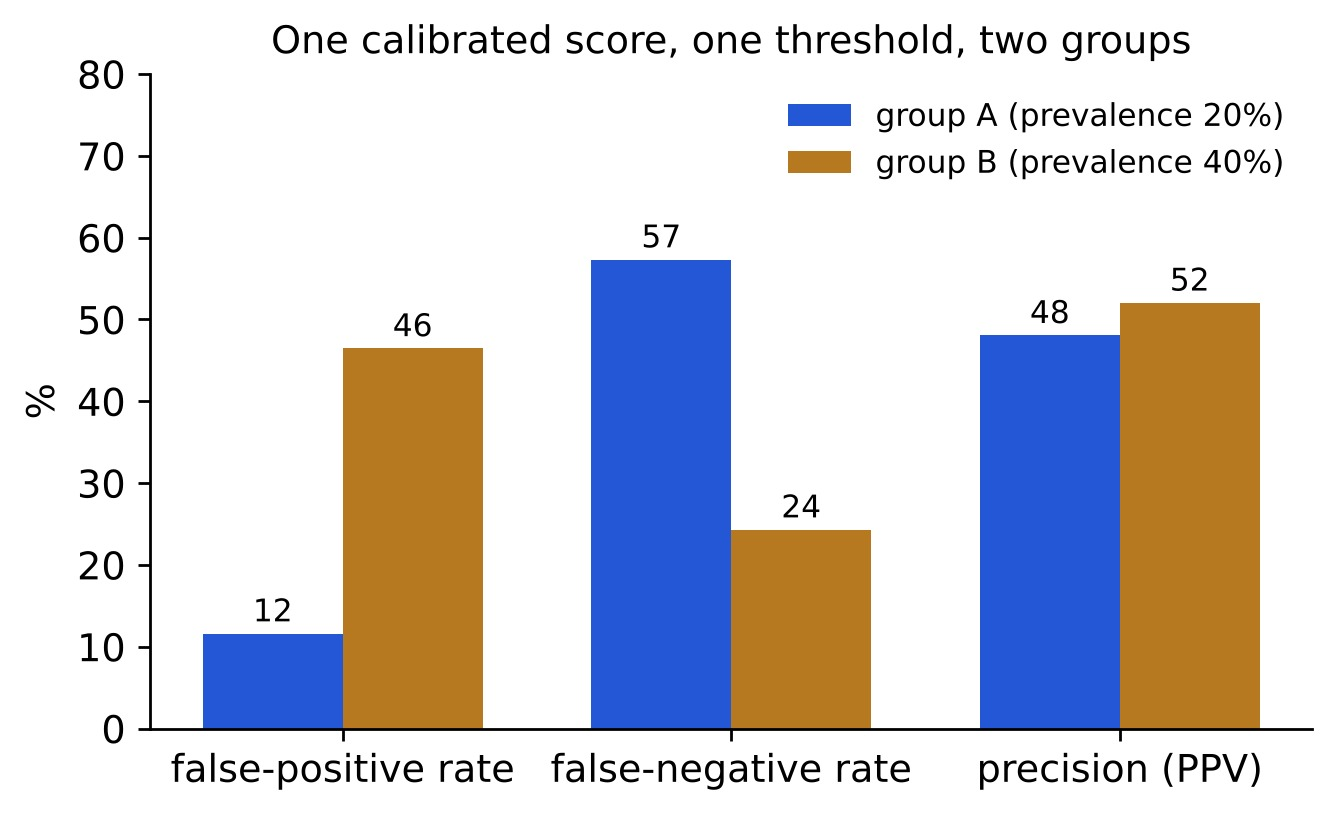
\includegraphics[width=\linewidth,height=0.6\textheight,keepaspectratio]{figs/hc_fair.jpg}\par
{\tiny Simulation: calibrated scores (Beta), prevalence 20\% vs 40\%, one threshold 0.35.}
\end{column}
\end{columns}
\srcc{Simulation written for this talk.}{hardt2016,kleinberg2017,chouldechova2017}
\end{frame}

\begin{frame}{Model \,|\, How sure: doubt that is honest for every group}
\chapstrip{1}
\begin{columns}[T]
\begin{column}{0.48\textwidth}
\fcard{tdAmber}{2018 \quad Evidential deep learning}{$p\sim\mathrm{Dir}(\alpha),\quad \alpha_k=e_k+1,\quad u=\dfrac{K}{\sum_k\alpha_k}$}{little evidence $\Rightarrow$ high doubt $u$, separately from a near tie}
\vspace{1mm}
{\footnotesize\textbf{Conformal sets} give $\mathbb P(Y\in\mathcal C(X))\ge1-\alpha$, also for survival times \cit{candes2023}. \bad{But the guarantee is marginal}: averaged over all patients.

\vspace{1mm}
\textbf{Fix:} calibrate per group (Mondrian). Each group then gets its own guarantee, and needs \key{its own calibration data}.}
\end{column}
\begin{column}{0.5\textwidth}
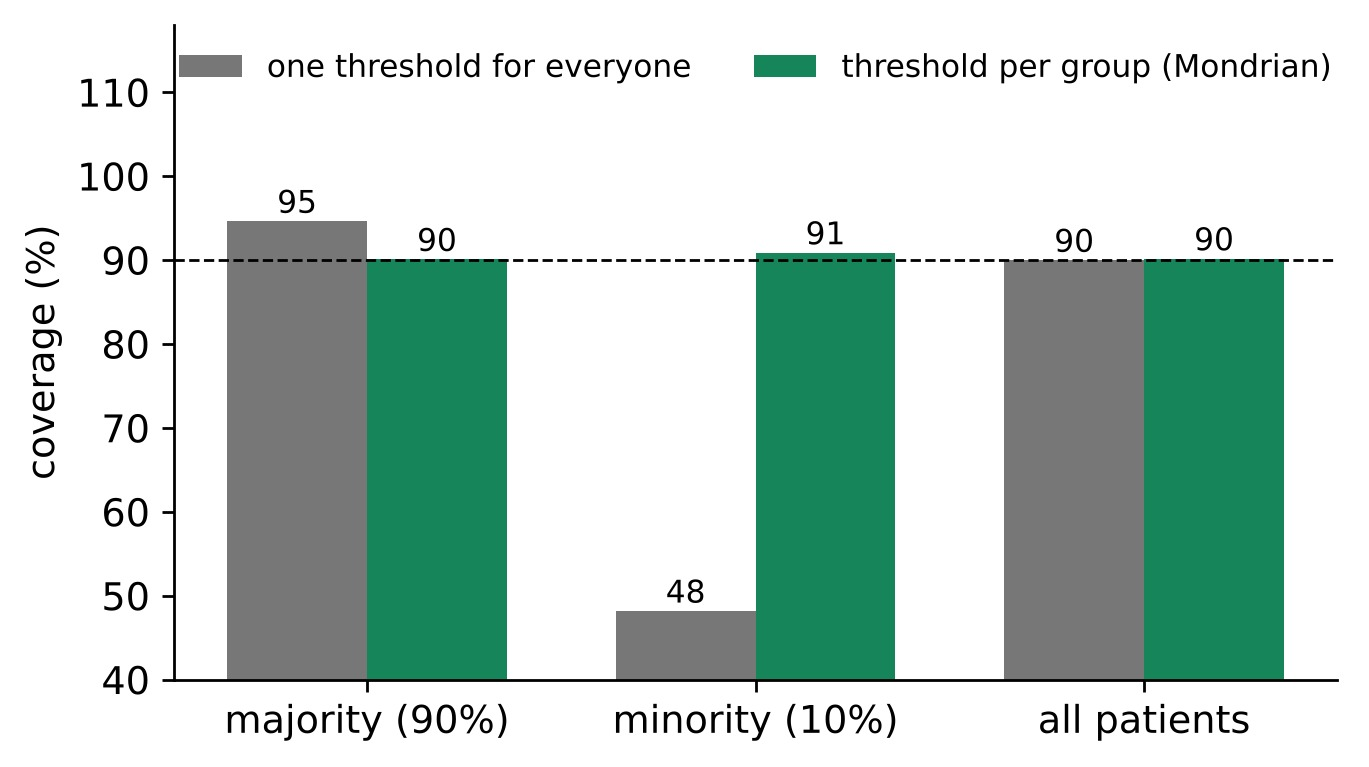
\includegraphics[width=\linewidth,height=0.58\textheight,keepaspectratio]{figs/hc_mondrian.jpg}\par
{\tiny Simulation: minority 10\% with noisier scores; 500 calibration patients; 2{,}000 repetitions; target 90\%.}
\end{column}
\end{columns}
\srcc{Simulation written for this talk.}{sensoy2018,begoli2019,candes2023,angelopoulos2023}
\end{frame}

\begin{frame}{Model \,|\, Putting it together: a trilemma}
\chapstrip{1}
\begin{columns}[T]
\begin{column}{0.56\textwidth}
\begin{sfig}[0.7]
\begin{tikzpicture}[x=1mm,y=1mm,font=\footnotesize]
  \node[card=tdBlue,minimum width=34mm] (p) at (0,52) {\textbf{Privacy}\\\scriptsize differential privacy};
  \node[card=tdGreen,minimum width=34mm] (f) at (-34,0) {\textbf{Fairness}\\\scriptsize equal error rates};
  \node[card=tdAmber,minimum width=34mm] (u) at (34,0) {\textbf{Uncertainty}\\\scriptsize calibrated, set-valued};
  \draw[thick,tdMuted] (p) -- (f); \draw[thick,tdMuted] (p) -- (u); \draw[thick,tdMuted] (f) -- (u);
  \node[lbl,text width=36mm,fill=tdPaper,inner sep=1pt] at (-24,28) {clipping and noise hurt \textbf{minority} groups most};
  \node[lbl,text width=36mm,fill=tdPaper,inner sep=1pt] at (26,28) {noise corrupts evidence and \textbf{quantiles}};
  \node[lbl,text width=40mm,fill=tdPaper,inner sep=1pt] at (0,-3) {group-wise coverage needs \textbf{enough samples} per group};
  \node[circle,draw=tdInk,fill=tdInk,text=white,font=\scriptsize\bfseries,inner sep=2pt,align=center] at (0,16) {clinical\\model};
\end{tikzpicture}
\end{sfig}
\end{column}
\begin{column}{0.42\textwidth}
{\footnotesize
\textbf{Privacy:} DP-SGD clips and noises gradients \cit{abadi2016}.\\[3pt]
\textbf{Fairness:} equal opportunity across groups \cit{hardt2016}; but differential privacy can have a \emph{disparate impact} on accuracy \cit{bagdasaryan2019}.\\[3pt]
\textbf{Uncertainty:} evidential networks \cit{sensoy2018}; conformal sets with coverage guarantees \cit{angelopoulos2023}.

\vspace{2mm}
Optimising one in isolation tends to break another.}
\end{column}
\end{columns}
\srcc{Our related work:}{abadi2016,bagdasaryan2019,angelopoulos2023,own2026cipherdifferentiallyprivate}
\end{frame}

\begin{frame}{Model \,|\, Our work: TRACER-Med, one model for all three}
\chapstrip{1}
\begin{sfig}[0.4]
\begin{tikzpicture}[node distance=4mm,font=\footnotesize]
  \node[card=tdPurple,text width=30mm] (e) {\textbf{Evidential} Dirichlet network\\{\scriptsize doubt = ignorance, not noise}};
  \node[card=tdBlue,text width=30mm,right=of e] (d) {\textbf{Subgroup-calibrated} DP-SGD\\{\scriptsize private, minority-aware clipping}};
  \node[card=tdGreen,text width=28mm,right=of d] (f) {\textbf{Prototype} alignment\\{\scriptsize fairness without per-sample leakage}};
  \node[card=tdAmber,text width=30mm,right=of f] (c) {\textbf{Private conformal} sets per group\\{\scriptsize coverage guarantees}};
  \foreach \p/\q in {e/d,d/f,f/c}{\draw[arr] (\p) -- (\q);}
  \node[card=tdRed,text width=100mm,below=5mm of d,xshift=18mm] (x) {\textbf{Dual-channel attribution:} separate \emph{what raises disease risk} from \emph{what raises clinical doubt}};
  \draw[arr] (c.south) |- (x.east);
\end{tikzpicture}
\end{sfig}
\vspace{3mm}

\begin{columns}[T]
\column{0.5\textwidth}{\footnotesize\textbf{Evaluated on} Statlog Heart ($N{=}270$), Pima Diabetes ($N{=}768$), a real 20,000-patient readmission cohort (UCI Diabetes 130-US Hospitals) and a simulated inpatient cohort ($N{=}10{,}000$).}
\column{0.46\textwidth}{\footnotesize\textbf{Against} ERM, DP-SGD, a fairness-aware DP method, PF-LD (adapted), evidential learning and DP-EDL, with an exact R\'enyi privacy accountant.}
\end{columns}
\srcc{TRACER-Med: our work in progress.}{abadi2016,sensoy2018}
\end{frame}

\begin{frame}{Model \,|\, TRACER-Med: what the experiments actually show}
\chapstrip{1}
\begin{columns}[c]
\column{0.32\textwidth}\begin{sfig}[0.55]\barpanel{Calibration error, 20k real cohort (lower is better)}{0.09}{0.018,0.079,0.080,0.039,0.011}\end{sfig}
\column{0.32\textwidth}\begin{sfig}[0.55]\barpanel{Equalized-odds gap, Pima (lower is better)}{0.30}{0.285,0.221,0.092,0.266,0.264}\end{sfig}
\column{0.32\textwidth}\begin{sfig}[0.55]\barpanel{Membership-inference AUC, Statlog Heart (0.5 = no leak)}{0.7}{0.611,0.539,0.521,0.543,0.523}\end{sfig}
\end{columns}
\vspace{2mm}

\begin{columns}[T]
\column{0.48\textwidth}{\footnotesize \good{Better:} calibration on the two larger cohorts (ECE 0.011--0.013 vs 0.026--0.080 for private baselines) and low membership-inference leakage, at a cost of about 0.02 ROC-AUC.}
\column{0.48\textwidth}{\footnotesize \bad{Not better:} fairness. On small cohorts the adapted PF-LD closes the equalized-odds gap more (0.09--0.11 vs 0.26 on Pima), and subgroup-calibrated clipping gave no consistent benefit.}
\end{columns}
\srcc{Results from our TRACER-Med experiments (default noise level; three-fold cross-validation). A numerical audit of the paper's own claims corrected several statements of an earlier version.}{}
\end{frame}

\begin{frame}{Model \,|\, Our work: small cohorts, where coverage guarantees fray}
\chapstrip{1}
\begin{columns}[T]
\begin{column}{0.54\textwidth}
\begin{sfig}[0.66]
\begin{tikzpicture}[x=1mm,y=1mm]
  \node[font=\small\bfseries,anchor=west] at (0,55) {Conformal survival: coverage at 90\% target};
  \draw[tdMuted] (6,0) -- (6,48); \draw[tdMuted] (6,0) -- (70,0);
  \foreach \v in {0,0.5,1.0}{\pgfmathsetmacro{\yy}{\v*45}\draw[tdLine] (6,\yy) -- (70,\yy);\node[font=\tiny,anchor=east] at (5,\yy) {\v};}
  \foreach \xx/\vv/\nm/\nn in {10/0.86/BMT/{$n{=}137$},31/0.67/Melanoma/{$n{=}205$},52/0.14/PBC/{$n{=}418$}}{
    \fill[tdBlue!70] (\xx,0) rectangle (\xx+14,\vv*45);
    \node[font=\scriptsize\bfseries,above] at (\xx+7,\vv*45) {\vv};
    \node[font=\tiny,align=center,below] at (\xx+7,0) {\nm\\\nn};}
  \draw[tdRed,thick,dashed] (6,40.5) -- (70,40.5) node[above left,font=\tiny,text=tdRed] {target 0.90};
\end{tikzpicture}
\end{sfig}
\end{column}
\begin{column}{0.43\textwidth}
{\footnotesize
\textbf{Preliminary} (our repository, public competing-risk datasets): the method ranks patients well (C-index 0.83 on PBC) yet \bad{misses the coverage target} with small calibration sets.

\vspace{2mm}
In TRACER-Med the PAC variant of the private conformal layer is \bad{vacuous below about 1,300 calibration records}.

\vspace{2mm}
\key{Lesson:} guarantees need data. Report calibration size, and fall back to clinician review when coverage cannot be certified.}
\end{column}
\end{columns}
\srcc{CONFIDE is published; the coverage experiments are preliminary results from our repository.}{own2026confideconformalfree,angelopoulos2023}
\end{frame}

\begin{frame}{Model \,|\, Hand-off: one hospital rarely has enough patients}
\chapstrip{1}
\centering
\begin{tikzpicture}[node distance=6mm]
  \node[card=tdBlue,text width=50mm,minimum height=20mm] (a) {\textbf{Every fix in this chapter needs data}\\[2pt]\small per-group calibration, privacy budgets, rare subgroups};
  \node[card=tdGreen,text width=50mm,minimum height=20mm,right=of a] (b) {\textbf{Data sit in many hospitals}\\[2pt]\small and law, ethics and trust keep them there};
  \draw[arr,very thick] (a) -- (b);
\end{tikzpicture}

\vspace{6mm}
{\footnotesize Next question: \key{can hospitals learn together without pooling records}, even when their data differ?}
\end{frame}

\begin{frame}{Collaborate \,|\, The simple solution, and federated learning}
\chapstrip{2}
\begin{columns}[T]
\begin{column}{0.48\textwidth}
{\footnotesize\textbf{Simple solution:} pool records in one data centre. \bad{Fails} on law, consent and institutional trust: medical data stay in silos \cit{rieke2020,kaissis2020}.}
\vspace{1mm}

\fcard{tdGreen}{2017 \quad Federated averaging}{$w_{t+1}=\sum_{k=1}^{K}\frac{n_k}{n}\,w^{(k)}_{t+1}$, \quad $w^{(k)}_{t+1}$ = local training from $w_t$}{models travel, records stay}
\end{column}
\begin{column}{0.49\textwidth}
{\footnotesize\good{It works in medicine:}
\begin{itemize}\setlength\itemsep{2pt}
\item 10 institutions, brain-tumour segmentation: about 99\% of the quality of a centrally trained model \cit{sheller2020};
\item 20 institutes on 5 continents predicted oxygen needs of COVID-19 patients, with better generalisation than single-site models \cit{dayan2021}.
\end{itemize}
\vspace{1mm}
\bad{But} FedAvg assumes the sites' data are alike. Hospitals differ in populations, devices, and even in how they \emph{code the label}.}
\end{column}
\end{columns}
\srcc{}{mcmahan2017,rieke2020,sheller2020,dayan2021}
\end{frame}

\begin{frame}{Collaborate \,|\, When sites differ: from drift corrections to clusters}
\chapstrip{2}
\begin{columns}[T]
\begin{column}{0.5\textwidth}
\fcard{tdAmber}{2020 \quad FedProx: stay near the global model}{$\min_w\ F_k(w)+\frac{\mu}{2}\|w-w_t\|^2$}{limits client drift; SCAFFOLD corrects it with control variates}
\vspace{1mm}
\fcard{tdBlue}{2020 \quad q-FFL: do not ignore the worst site}{$\min_w\ \sum_k \frac{p_k}{q+1}F_k(w)^{q+1}$}{larger $q$ weights high-loss sites more}
\vspace{1mm}
\fcard{tdGreen}{2020--2021 \quad Clustered FL}{$\hat c_k=\arg\min_j F_k(\theta_j)$, train one model per cluster}{sites that genuinely disagree get different models}
\end{column}
\begin{column}{0.48\textwidth}
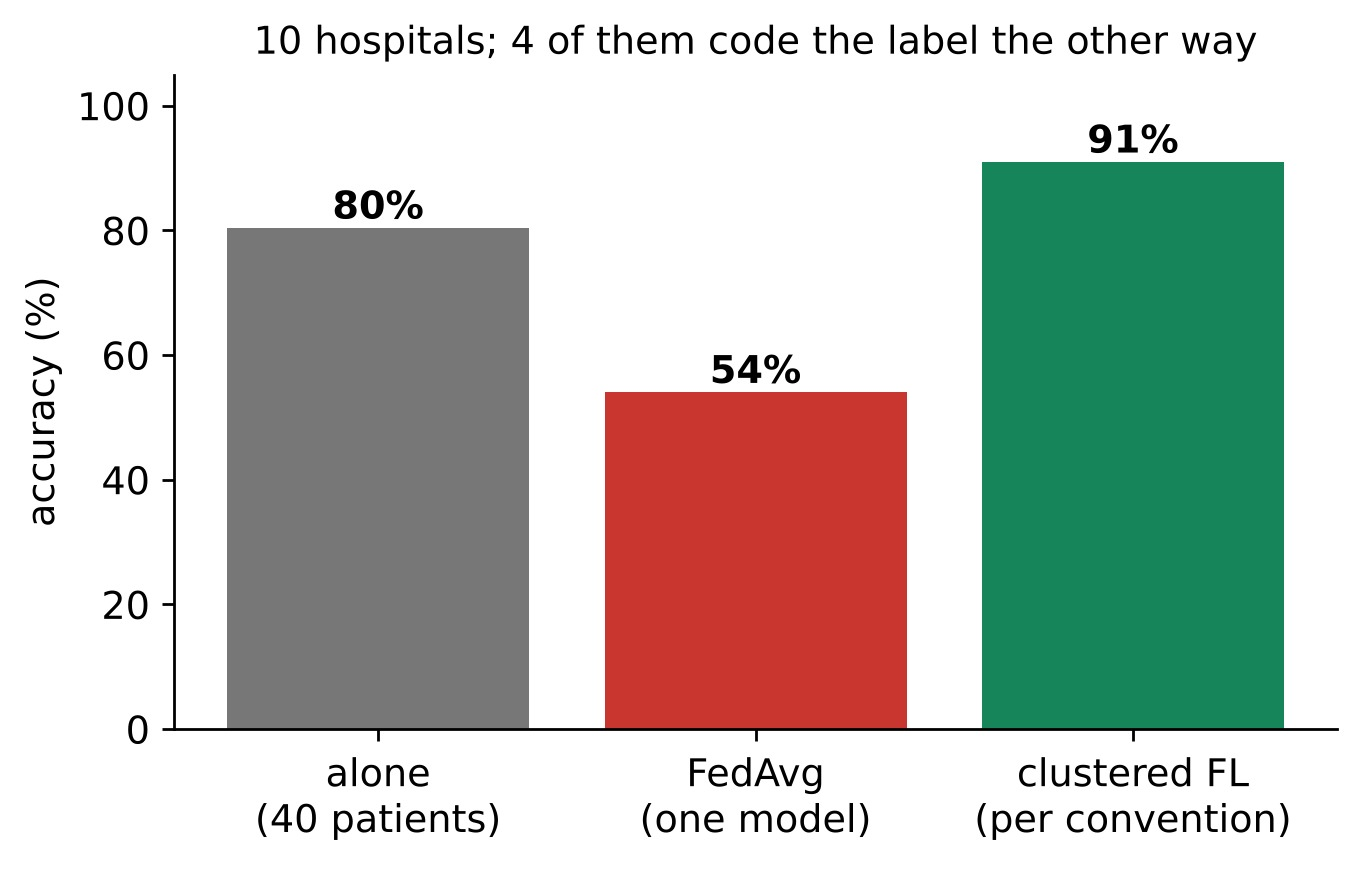
\includegraphics[width=\linewidth,height=0.5\textheight,keepaspectratio]{figs/hc_fl.jpg}\par
{\tiny Simulation: 20-feature logistic task; 6 sites use one label convention, 4 the opposite; 40 patients per site; 20 repetitions.}
\end{column}
\end{columns}
\srcc{Simulation written for this talk.}{li2020fedprox,karimireddy2020,li2020qffl,ghosh2020,sattler2021}
\end{frame}

\begin{frame}{Collaborate \,|\, Our work: fair, private and robust federated learning on graphs}
\chapstrip{2}
\begin{columns}[T]
\begin{column}{0.52\textwidth}
\begin{sfig}[0.7]
\begin{tikzpicture}[x=1mm,y=1mm,font=\footnotesize]
  \node[font=\small\bfseries,anchor=west] at (0,55) {Demographic-parity gap (budget 0.03)};
  \draw[tdMuted] (6,0) -- (6,48); \draw[tdMuted] (6,0) -- (70,0);
  \foreach \v in {0,0.04,0.08}{\pgfmathsetmacro{\yy}{\v*500}\draw[tdLine] (6,\yy) -- (70,\yy);\node[font=\tiny,anchor=east] at (5,\yy) {\v};}
  \foreach \xx/\a/\b/\nm in {8/0.071/0.018/{graph 1},28/0.042/0.026/{graph 2},48/0.052/0.028/{graph 3}}{
    \fill[tdMuted!55] (\xx,0) rectangle (\xx+8,\a*500); \fill[tdBlue!75] (\xx+9,0) rectangle (\xx+17,\b*500);
    \node[font=\tiny,above] at (\xx+4,\a*500) {\a}; \node[font=\tiny,above] at (\xx+13,\b*500) {\b};
    \node[font=\tiny,below] at (\xx+8.5,0) {\nm};}
  \draw[tdRed,dashed,thick] (6,15) -- (70,15);
  \node[font=\tiny,text=tdMuted!70!black,anchor=west] at (36,46) {grey: no fairness control};
  \node[font=\tiny,text=tdBlue,anchor=west] at (36,42) {blue: with fairness control};
\end{tikzpicture}
\end{sfig}
\end{column}
\begin{column}{0.45\textwidth}
{\footnotesize
\textbf{Idea:} the server sees only validated sums. One broadcast multiplier enforces a parity budget; secure aggregation and noise protect the statistics.

\vspace{2mm}
\good{Result:} gaps cut to 0.018--0.028 at AUC within 0.01. Under fairness poisoning: 0.025--0.049 vs 0.11--0.20 for FedAvg.

\vspace{2mm}
\bad{Limits:} loose Byzantine bounds; fails on small graphs; one falsified client can switch it off.}
\end{column}
\end{columns}
\srcc{Follow-up (CLAMP): our work in progress; fraud and social graphs, not clinical data.}{dang2026fedfairgnn,hardt2016}
\end{frame}

\begin{frame}{Collaborate \,|\, Our work: DisCo-CFL, group sites by \emph{concept}}
\chapstrip{2}
\begin{columns}[T]
\begin{column}{0.5\textwidth}
\begin{sfig}[0.62]
\begin{tikzpicture}[x=1mm,y=1mm,font=\footnotesize]
  \foreach \i/\xx/\cc in {1/6/tdBlue,2/24/tdBlue,3/42/tdRed,4/60/tdRed}{
    \node[card=\cc,minimum width=13mm,font=\scriptsize] (c\i) at (\xx,30) {site \i};}
  \node[font=\scriptsize,text=tdBlue!70!black] at (15,40) {coding A};
  \node[font=\scriptsize,text=tdRed] at (51,40) {coding B (labels swapped)};
  \node[card=tdAmber,minimum width=60mm,font=\scriptsize] (s) at (33,10) {one count-sketched gradient per class, once};
  \foreach \i in {1,2,3,4}{\draw[arr] (c\i) -- (s);}
  \node[card=tdGreen,minimum width=60mm,font=\scriptsize] at (33,-6) {calibrated similarity $\rightarrow$ clusters, with a certificate};
  \draw[arr] (s) -- (33,-1);
\end{tikzpicture}
\end{sfig}
\end{column}
\begin{column}{0.47\textwidth}
{\footnotesize
Sites may share images but \emph{label them differently} (coding conventions). Averaging them hurts everyone.

\vspace{2mm}
\textbf{Result:} groups recovered (ARI 0.94--1.00) on small image benchmarks; on CIFAR-100 with label-swap groups \good{63.0\%} vs \bad{55.5\%} for FedAvg.

\vspace{2mm}
\bad{Fails} to separate groups on Office-Home and rotated CIFAR-100, where clustering gains under one point.}
\end{column}
\end{columns}
\srcc{DisCo-CFL: our work in progress. Clustered federated learning:}{sattler2021,ghosh2020}
\end{frame}

\begin{frame}{Collaborate \,|\, Hand-off: models remember what they saw}
\chapstrip{2}
\centering
\begin{tikzpicture}[node distance=6mm]
  \node[card=tdGreen,text width=50mm,minimum height=20mm] (a) {\textbf{Federated learning keeps records local}\\[2pt]\small but the shared model is trained on them};
  \node[card=tdAmber,text width=50mm,minimum height=20mm,right=of a] (b) {\textbf{A model is a compressed copy of its data}\\[2pt]\small which an attacker can query};
  \draw[arr,very thick] (a) -- (b);
\end{tikzpicture}

\vspace{6mm}
{\footnotesize Next question: \key{what can be learned about a patient from the data or the model}, and can a patient be \emph{forgotten}?}
\end{frame}

\begin{frame}{Data owner \,|\, The simple solution: remove the names}
\chapstrip{3}
\begin{columns}[T]
\begin{column}{0.52\textwidth}
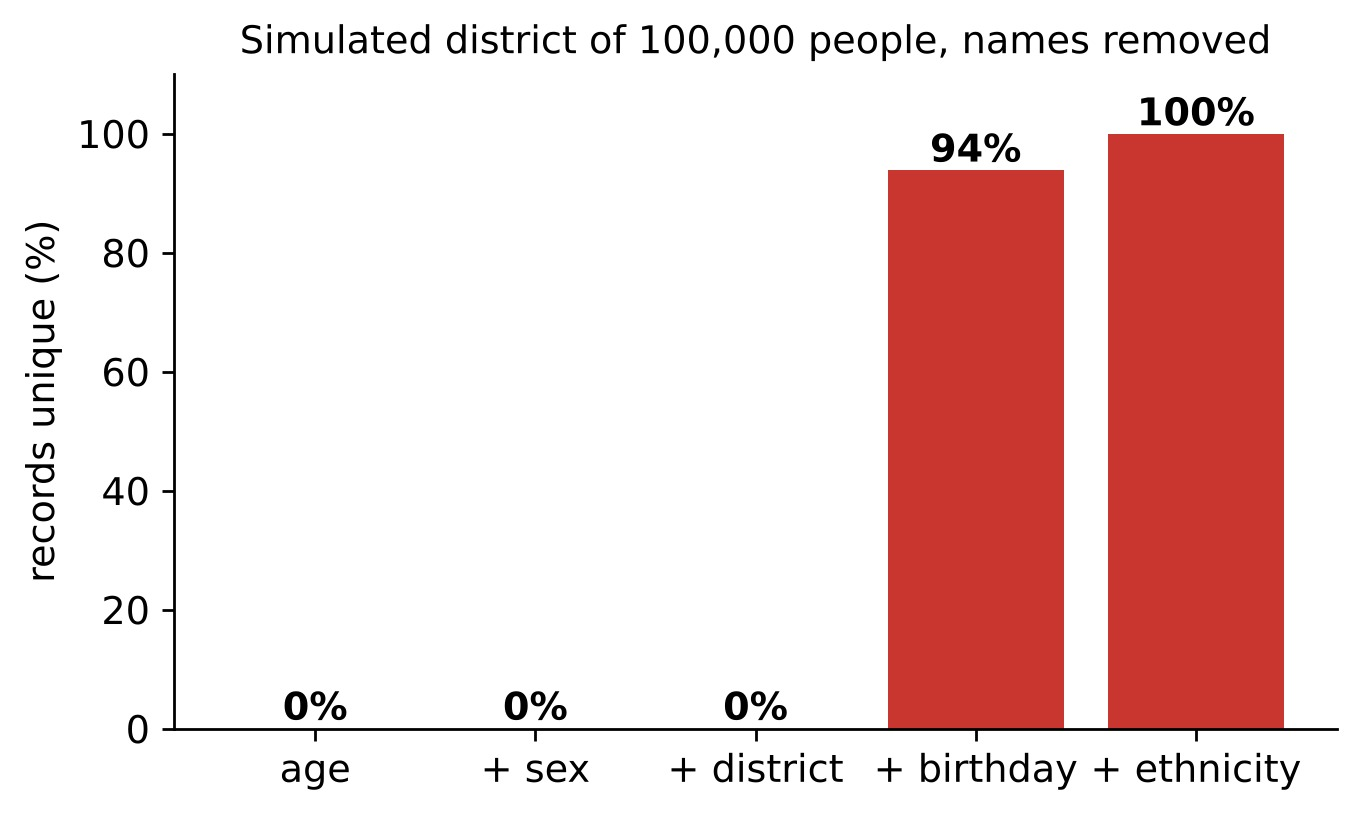
\includegraphics[width=\linewidth,height=0.5\textheight,keepaspectratio]{figs/hc_reid.jpg}\par
{\tiny Simulation: 100{,}000 synthetic residents; age 18--89, sex, 30 districts, day of birth, 54 ethnic groups (uniform).}
\end{column}
\begin{column}{0.45\textwidth}
{\footnotesize\bad{Fails quickly.} A few ordinary attributes make most people unique, so a ``de-identified'' record can be linked back to a name. Sweeney reported that ZIP code, sex and date of birth likely identify 87\% of the US population, and proposed $k$-anonymity \cit{sweeney2002}.

\vspace{2mm}
Sparse records are worse: a handful of ratings re-identified Netflix users \cit{narayanan2008}.

\vspace{2mm}
In genomics, even \textbf{aggregate} statistics revealed whether a person's DNA was in a study mixture \cit{homer2008}.}
\end{column}
\end{columns}
\srcc{Simulation written for this talk.}{sweeney2002,narayanan2008,homer2008}
\end{frame}

\begin{frame}{Data owner \,|\, Development: the model itself leaks, so audit it}
\chapstrip{3}
\begin{columns}[T]
\begin{column}{0.5\textwidth}
\fcard{tdAmber}{2017 \quad Membership inference}{$\mathrm{Adv}=\mathbb P(\text{guess in}\mid\text{in})-\mathbb P(\text{guess in}\mid\text{out})$}{was this patient in the training set? shadow models answer it}
\vspace{1mm}
{\footnotesize\textbf{2021:} language models emit memorised training text verbatim, including personal data \cit{carlini2021}.

\vspace{1mm}
\textbf{Defences:} differential privacy bounds the advantage; \textbf{canaries} measure it in practice \cit{carlini2019,steinke2023}.}
\end{column}
\begin{column}{0.47\textwidth}
{\footnotesize\textbf{The right to erasure} (GDPR, Art.~17) meets models trained on the data \cit{gdpr2016}. Machine unlearning makes deletion cheaper, e.g.\ by retraining only one shard (SISA) \cit{bourtoule2021}.}
\vspace{2mm}
\begin{alertblock}{The missing piece}
{\footnotesize The patient or hospital cannot inspect the model, and the operator has no incentive to report failure. \textbf{How can forgetting be verified?} And before that: \textbf{how much does a shard of data disclose?}}
\end{alertblock}
\end{column}
\end{columns}
\srcc{}{shokri2017,carlini2021,steinke2023,bourtoule2021,own2021rightbeforgotten}
\end{frame}

\begin{frame}{Data owner \,|\, Our work: SHADE, what can be reconstructed from the pieces?}
\chapstrip{3}
\begin{columns}[T]
\begin{column}{0.54\textwidth}
\begin{sfig}[0.68]
\begin{tikzpicture}[x=1mm,y=1mm,font=\footnotesize]
  \node[card=tdBlue,minimum width=26mm,minimum height=26mm] (k) at (0,24) {sensitive\\knowledge\\base};
  \foreach \i/\yy/\cc in {1/46/tdAmber,2/24/tdGreen,3/2/tdPurple}{
    \node[card=\cc,minimum width=30mm,font=\scriptsize] (p\i) at (58,\yy) {shard \i $\rightarrow$ LLM provider \i};
    \draw[arr] (k.east) -- (p\i.west);}
  \node[lbl,text width=40mm] at (58,-9) {each provider answers queries; none may reconstruct the whole};
\end{tikzpicture}
\end{sfig}
\end{column}
\begin{column}{0.43\textwidth}
{\footnotesize
\textbf{SHADE} measures the \emph{semantic disclosure} of a shard: an axiomatised measure with an LLM-oracle form and a cheap embedding-coverage proxy.

\vspace{2mm}
\textbf{CoShard} partitions the corpus on a graph, adding the disclosure penalty to trace the \key{coherence versus secrecy} frontier.

\vspace{2mm}
Datasets include a synthetic HR corpus, \textbf{MedQA} and LegalBench.}
\end{column}
\end{columns}
\srcc{SHADE and CoShard: our work in progress (code released).}{carlini2021,shokri2017}
\end{frame}

\begin{frame}{Data owner \,|\, Our work: VOUCH, the protocol in one picture}
\chapstrip{3}
\centering
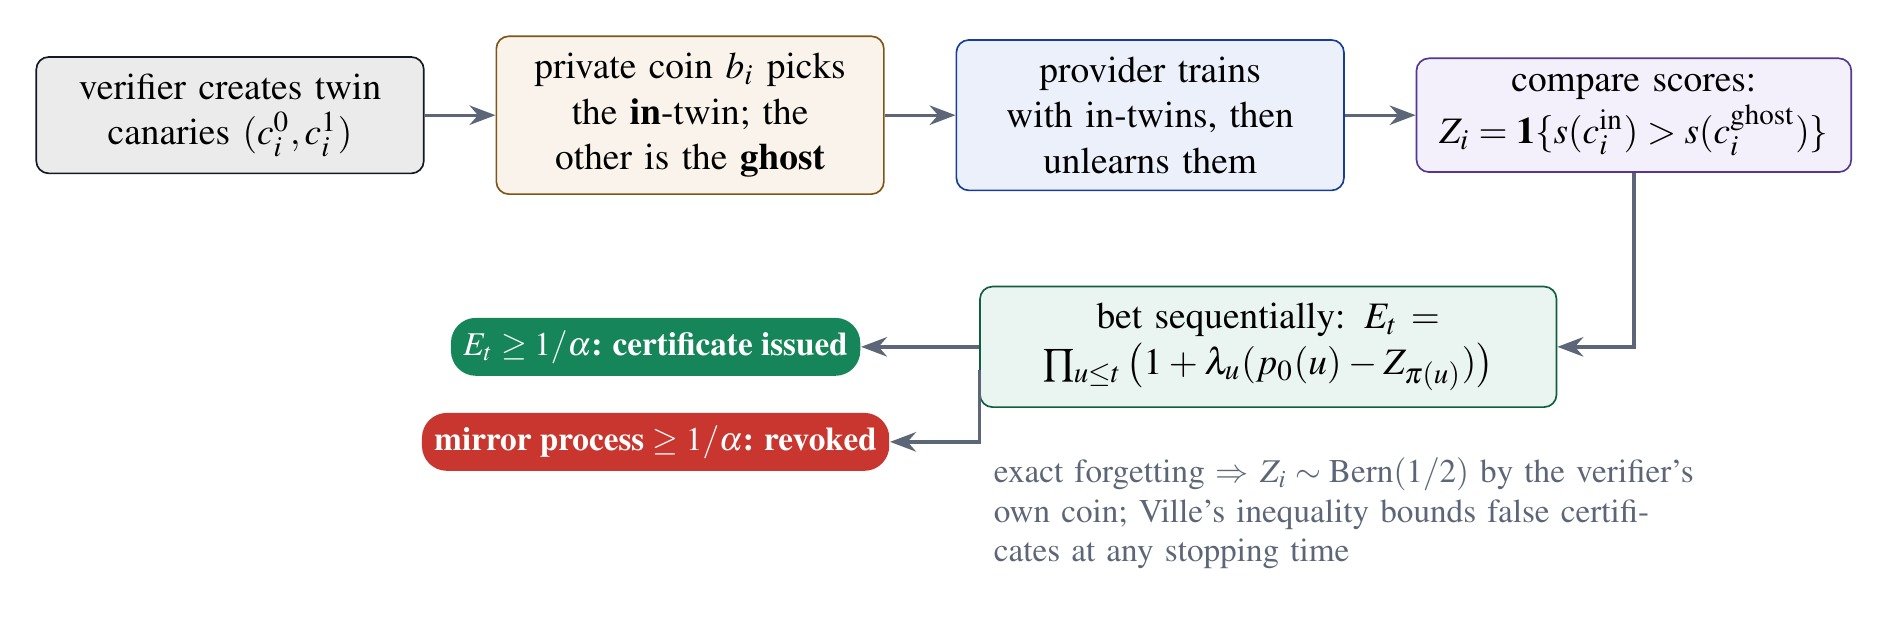
\includegraphics[width=\linewidth,height=0.62\textheight,keepaspectratio]{figs/vouch_protocol.jpg}

{\footnotesize Canaries from privacy auditing + betting from sequential testing: a certificate that the \key{data owner} can check, valid at any stopping time.}
\srcc{Accepted, Machine Learning.}{dang2026vouch,steinke2023,ramdas2023}
\end{frame}

\begin{frame}{Data owner \,|\, Our work: auditing erasure under mutual distrust}
\chapstrip{3}
\begin{columns}[T]
\begin{column}{0.5\textwidth}
\begin{sfig}[0.46]
\begin{tikzpicture}[x=1mm,y=1mm,font=\footnotesize]
  \node[card=tdBlue,minimum width=18mm] (a) at (6,32) {twin A};
  \node[card=tdBlue,minimum width=18mm] (b) at (6,10) {twin B};
  \node[circle,draw=tdInk,fill=white,font=\scriptsize,align=center,inner sep=1pt] (coin) at (30,21) {fair\\coin};
  \draw[arr] (a) -- (coin); \draw[arr] (b) -- (coin);
  \node[card=tdGreen,minimum width=26mm] (t) at (60,32) {one is \textbf{trained on}};
  \node[card=tdAmber,minimum width=26mm] (g) at (60,10) {one is a \textbf{ghost}};
  \draw[arr] (coin) -- (t); \draw[arr] (coin) -- (g);
  \node[card=tdPurple,minimum width=48mm] (u) at (40,-8) {after unlearning, scores must be \textbf{symmetric}};
  \draw[arr,dashed] (t.east) -- ++(6,0) |- (u.east);
\end{tikzpicture}
\end{sfig}
\vspace{1mm}

{\footnotesize \textbf{VOUCH:} un-unlearned models revoked in \good{16/18} runs; retraining, gradient ascent and NPO certified 18/18 at $\varepsilon=0.2$.}
\end{column}
\begin{column}{0.47\textwidth}
\begin{sfig}[0.4]
\begin{tikzpicture}[x=1mm,y=1mm]
  \node[font=\small\bfseries,anchor=west] at (0,52) {SEAL-W: catching an operator who filters the audit query};
  \draw[tdMuted] (6,0) -- (6,44); \draw[tdMuted] (6,0) -- (60,0);
  \foreach \v in {0,0.5,1.0}{\pgfmathsetmacro{\yy}{\v*40}\draw[tdLine] (6,\yy) -- (60,\yy);\node[font=\tiny,anchor=east] at (5,\yy) {\v};}
  \fill[tdRed!70] (12,0) rectangle (26,0.4); \node[font=\scriptsize\bfseries,above] at (19,0.4) {0\%};
  \fill[tdGreen!70] (36,0) rectangle (50,0.93*40); \node[font=\scriptsize\bfseries,above] at (43,0.93*40) {93\%};
  \node[font=\tiny,align=center,below] at (19,0) {single-query\\check};\node[font=\tiny,align=center,below] at (43,0) {full\\SEAL-W};
\end{tikzpicture}
\end{sfig}
\vspace{1mm}

{\footnotesize \bad{Honest note:} a composition bound was \emph{violated in our own code} and fixed by writing the proof. The audit has little power for small models.}
\end{column}
\end{columns}
\srcc{VOUCH: accepted in Machine Learning. SEAL: our work in progress.}{dang2026vouch,bourtoule2021,own2021rightbeforgotten}
\end{frame}

\begin{frame}{Data owner \,|\, Hand-off: from stored data to generated answers}
\chapstrip{3}
\centering
\begin{tikzpicture}[node distance=6mm]
  \node[card=tdAmber,text width=50mm,minimum height=20mm] (a) {\textbf{So far the risk sat in the data}\\[2pt]\small what leaks, what is remembered};
  \node[card=tdRed,text width=50mm,minimum height=20mm,right=of a] (b) {\textbf{Assistants act on what they read}\\[2pt]\small and write text that clinicians may trust};
  \draw[arr,very thick] (a) -- (b);
\end{tikzpicture}

\vspace{6mm}
{\footnotesize Last question: \key{are an assistant's answers grounded}, and \key{can it be steered} by what it reads?}
\end{frame}

\begin{frame}{Assistant \,|\, The simple solution: a large model that knows medicine}
\chapstrip{4}
\begin{columns}[T]
\begin{column}{0.5\textwidth}
\begin{sfig}[0.62]
\begin{tikzpicture}[node distance=4mm,font=\footnotesize]
  \node[card=tdBlue,text width=26mm] (u) {{\large\faUserMd}\\ question + image};
  \node[card=tdPurple,text width=26mm,right=of u] (a) {{\large\faRobot}\\ assistant};
  \node[card=tdAmber,text width=26mm,below=8mm of a] (k) {{\large\faFileMedical}\\ records, guidelines, web};
  \node[card=tdGreen,text width=26mm,right=of a] (o) {{\large\faClipboardCheck}\\ answer};
  \draw[arr] (u) -- (a); \draw[arr] (a) -- (o); \draw[<->,thick,tdMuted] (a) -- (k);
  \node[pill=tdRed,left=3mm of k] {hidden instruction};
  \node[pill=tdRed,above=3mm of o] {fabricated finding};
\end{tikzpicture}
\end{sfig}
\end{column}
\begin{column}{0.47\textwidth}
{\footnotesize\textbf{2023:} a large language model reached passing level on medical licensing questions; judging it also needed clinician review of factuality and harm \cit{singhal2023}.

\vspace{2mm}
\bad{Three ways it breaks:}
\begin{itemize}\setlength\itemsep{1pt}
\item \textbf{hallucination}: fluent, unsupported content \cit{ji2023};
\item \textbf{poisoning}: replacing 0.001\% of training tokens with medical misinformation produced more harmful models that standard benchmarks did not flag \cit{alber2025};
\item \textbf{injection}: hidden instructions in images hijacked medical VLMs \cit{clusmann2025}.
\end{itemize}}
\end{column}
\end{columns}
\srcc{}{singhal2023,ji2023,alber2025,clusmann2025}
\end{frame}

\begin{frame}{Assistant \,|\, Development: ground the answer, then control the risk}
\chapstrip{4}
\begin{columns}[T]
\begin{column}{0.5\textwidth}
\begin{sfig}[0.62]
\begin{tikzpicture}
\begin{axis}[width=7.8cm,height=5.4cm,xlabel={share of questions answered},ylabel={error among answered},xmin=0,xmax=1,ymin=0,ymax=0.22,axis lines=left]
  \addplot[domain=0:1,samples=60,very thick,tdBlue] {0.02+0.18*x^3};
  \addplot[tdRed,dashed] coordinates {(0,0.05)(1,0.05)};
  \addplot[tdGreen,very thick] coordinates {(0.55,0)(0.55,0.05)};
  \node[font=\tiny,text=tdRed,anchor=south west] at (axis cs:0.02,0.051) {target risk $\alpha$};
  \node[font=\tiny,text=tdGreen!70!black,anchor=west] at (axis cs:0.57,0.02) {answer 55\%, defer the rest};
\end{axis}
\end{tikzpicture}
\end{sfig}
{\tiny\illus\ risk--coverage curve}
\end{column}
\begin{column}{0.47\textwidth}
{\footnotesize\textbf{Grounding:} retrieve evidence and generate from it (RAG) \cit{lewis2020}; check outputs against it.

\vspace{1mm}
\textbf{Selective answering with a guarantee:} choose the confidence threshold $\hat\lambda$ on calibration data so that
\[\mathbb E\big[\ell(Y,\mathcal C_{\hat\lambda}(X))\big]\le\alpha\]
with high probability \cit{bates2021,angelopoulos2024crc}; or drop sub-claims until the rest is factual with probability $\ge1-\alpha$ \cit{mohri2024}.

\vspace{1mm}
\bad{The price:} deferral. In a clinic, a deferral is a task for a busy clinician.}
\end{column}
\end{columns}
\srcc{}{lewis2020,bates2021,angelopoulos2024crc,mohri2024}
\end{frame}

\begin{frame}{Assistant \,|\, Our work: CMVKG-Guard, correct while the model writes}
\chapstrip{4}
\begin{sfig}[0.40]
\begin{tikzpicture}[node distance=5mm,font=\footnotesize]
  \node[card=tdPurple,text width=24mm] (v) {\textbf{VLM} writes token by token};
  \node[card=tdBlue,text width=38mm,right=of v] (k) {\textbf{scene knowledge graph}\\from the image\\+ Wikidata, ConceptNet};
  \node[card=tdAmber,text width=44mm,right=of k] (x) {\textbf{three-layer check}\\visual--text 30\% $\cdot$ graph 40\% $\cdot$ reasoning 30\%};
  \node[card=tdGreen,text width=36mm,right=of x] (s) {\textbf{replace} low-score tokens with grounded ones};
  \foreach \p/\q in {v/k,k/x,x/s}{\draw[arr] (\p) -- (\q);}
\end{tikzpicture}
\end{sfig}
\vspace{2mm}

\begin{columns}[T]
\column{0.3\textwidth}\centering{\huge\bfseries\color{tdGreen!70!black}84\%}\\[-1pt]{\scriptsize fewer object hallucinations (CHAIR)}
\column{0.3\textwidth}\centering{\huge\bfseries\color{tdGreen!70!black}91.2}\\[-1pt]{\scriptsize F1 on POPE (base model 82.1)}
\column{0.3\textwidth}\centering{\huge\bfseries\color{tdGreen!70!black}12\,ms}\\[-1pt]{\scriptsize extra latency per token}
\end{columns}
\vspace{2mm}

{\footnotesize Training-free, so it can wrap a deployed model. \bad{Not yet tested} on radiology images or clinical reports: general-domain benchmarks only.}
\srcc{Six benchmarks, eight baselines.}{own2026realtimehallucination,pope2023,ji2023}
\end{frame}

\begin{frame}{Assistant \,|\, Our work: CCRC, can a correction be \emph{certified}?}
\chapstrip{4}
\begin{columns}[T]
\begin{column}{0.52\textwidth}
\begin{sfig}[0.66]
\begin{tikzpicture}
\begin{axis}[width=8cm,height=5.4cm,xlabel={base error rate $\mu$},ylabel={forced abstention},xmin=0,xmax=0.6,ymin=0,ymax=0.7,axis lines=left]
  \addplot[domain=0.05:0.6,very thick,tdRed,samples=40] {(x-0.05)/(1-0.05)};
  \node[font=\scriptsize,text=tdRed,anchor=east] at (axis cs:0.58,0.28) {emit-or-abstain only};
  \node[font=\scriptsize,anchor=west] at (axis cs:0.02,0.62) {target error $\alpha=0.05$};
\end{axis}
\end{tikzpicture}
\end{sfig}
\end{column}
\begin{column}{0.45\textwidth}
{\footnotesize
\textbf{Impossibility:} a model that can only emit its own answer or abstain must refuse at least $(\mu-\alpha)/(1-\alpha)$ of inputs when $\mu>\alpha$.

\vspace{2mm}
\textbf{CCRC} may also \key{substitute} an answer from an independent evidence channel and certifies the error of everything emitted.

\vspace{2mm}
\good{Honest finding:} against a similarity-based scorer, most of the coverage gain comes from a better correctness \emph{score}; certified repair adds a few points.

\vspace{2mm}
\bad{Scope:} general vision-language benchmarks.}
\end{column}
\end{columns}
\srcc{CCRC: our work in progress (five benchmarks, two backbones, 400+ paired splits).}{bates2021,angelopoulos2024crc}
\end{frame}

\begin{frame}{Assistant \,|\, Our work: watch the trace, recalibrate the guards}
\chapstrip{4}
\begin{columns}[T]
\begin{column}{0.5\textwidth}
\begin{sfig}[0.4]
\begin{tikzpicture}[x=1mm,y=1mm]
  \node[font=\small\bfseries,anchor=west] at (0,52) {SENTRY-Fuse: recall at 5\% false alarms};
  \draw[tdMuted] (6,0) -- (6,44); \draw[tdMuted] (6,0) -- (66,0);
  \foreach \v in {0,0.5,1.0}{\pgfmathsetmacro{\yy}{\v*42}\draw[tdLine] (6,\yy) -- (66,\yy);\node[font=\tiny,anchor=east] at (5,\yy) {\v};}
  \fill[tdAmber!70] (12,0) rectangle (28,{0.709*42}); \draw[thick,tdAmber!60!black] (20,{(0.709-0.357)*42}) -- (20,{(0.709+0.357)*42});
  \node[font=\scriptsize\bfseries,anchor=west] at (29,{0.709*42}) {0.71$\pm$0.36};
  \fill[tdGreen!70] (40,0) rectangle (56,{0.898*42}); \draw[thick,tdGreen!60!black] (48,{(0.898-0.02)*42}) -- (48,{(0.898+0.02)*42});
  \node[font=\scriptsize\bfseries,anchor=south] at (48,{(0.898+0.02)*42+1}) {0.90$\pm$0.02};
  \node[font=\scriptsize,align=center] at (20,-6) {one signal};\node[font=\scriptsize,align=center] at (48,-6) {SENTRY-Fuse};
\end{tikzpicture}
\end{sfig}
\vspace{1mm}

{\footnotesize Flags a hijacked agent from its action trace (90 traces). The gain is mostly \key{stability}.}
\end{column}
\begin{column}{0.47\textwidth}
\begin{sfig}[0.4]
\begin{tikzpicture}[x=1mm,y=1mm]
  \node[font=\small\bfseries,anchor=west] at (0,52) {Activation-gated guards, new framings};
  \draw[tdMuted] (6,0) -- (6,44); \draw[tdMuted] (6,0) -- (66,0);
  \foreach \v in {0,50,100}{\pgfmathsetmacro{\yy}{\v*0.42}\draw[tdLine] (6,\yy) -- (66,\yy);\node[font=\tiny,anchor=east] at (5,\yy) {\v\%};}
  \fill[tdRed!25] (12,0) rectangle (28,{17*0.42}); \fill[tdRed!75] (12,0) rectangle (28,{0*0.42+0.4});
  \node[font=\scriptsize\bfseries,anchor=south] at (20,{17*0.42}) {0--17\%};
  \fill[tdGreen!25] (40,{83*0.42}) rectangle (56,{94*0.42}); \fill[tdGreen!75] (40,0) rectangle (56,{83*0.42});
  \node[font=\scriptsize\bfseries,anchor=south] at (48,{94*0.42}) {83--94\%};
  \node[font=\scriptsize,align=center] at (20,-6) {as designed};\node[font=\scriptsize,align=center] at (48,-6) {recalibrated};
\end{tikzpicture}
\end{sfig}
\vspace{1mm}

{\footnotesize Recall at 1\% false positives on \emph{withheld} jailbreak framings. The signal remains (AUROC 0.95--1.00); the \bad{threshold} was miscalibrated.}
\end{column}
\end{columns}
\srcc{SENTRY-Fuse and the activation-gate study: our work in progress.}{greshake2023,debenedetti2024,clusmann2025}
\end{frame}

\begin{frame}{An integrated view: evaluate all four properties at every stage}
\footnotesize\renewcommand{\arraystretch}{1.08}
\begin{tabularx}{\textwidth}{@{}>{\raggedright\bfseries}p{26mm}>{\centering}X>{\centering}X>{\centering}X>{\centering\arraybackslash}X@{}}
\toprule
\normalsize Stage & \normalsize Privacy & \normalsize Fairness & \normalsize Uncertainty & \normalsize Security\\
\midrule
Data and training & \textcolor{tdBlue}{DP-SGD, SC-DP} (TRACER-Med) & subgroup clipping, prototypes & evidential doubt & poisoning checks\\
Collaboration & secure aggregation, DP statistics & parity budget (FedFairGNN) & site-level coverage & Byzantine-robust (FORTRESS-FL)\\
Disclosure and erasure & disclosure score (SHADE) & -- & anytime-valid certificates (VOUCH) & erasure audits (SEAL)\\
Deployment and assistants & -- & -- & certified selective answers (CCRC) & trace monitors (SENTRY), guards\\
\bottomrule
\end{tabularx}

\vspace{1mm}
{\scriptsize \faHeartbeat\ validated on \textbf{biomedical} data: TRACER-Med, CONFIDE \quad \faProjectDiagram\ validated on \textbf{other domains}: federated graphs, FL, assistants \quad \faHandshake\ \textbf{needs validation} with healthcare partners}
\end{frame}

\begin{frame}{The common thread}
\centering
\begin{sfig}[0.62]
\begin{tikzpicture}[x=1mm,y=1mm,font=\footnotesize]
  \foreach \yy/\cc/\q/\simple/\now/\check in {
     36/tdBlue/{Model}/{average loss, one AUC}/{DP, fairness criteria, conformal}/{per-group guarantees},
     24/tdGreen/{Collaborate}/{pool the data}/{FedAvg, FedProx, clusters}/{fair, robust aggregation},
     12/tdAmber/{Data owner}/{remove names}/{DP, membership audits, unlearning}/{erasure certificates},
     0/tdRed/{Assistant}/{trust the fluent answer}/{RAG, risk control}/{certified answers, monitors}}{
    \node[pill=\cc,minimum width=20mm] at (0,\yy) {\q};
    \node[card=tdMuted,text width=30mm,minimum height=7mm] (a) at (35,\yy) {\simple};
    \node[card=\cc,text width=38mm,minimum height=7mm] (b) at (80,\yy) {\now};
    \node[card=tdGreen,text width=32mm,minimum height=7mm] (c) at (124,\yy) {\check};
    \draw[arr] (a) -- (b); \draw[arr] (b) -- (c);}
  \node[font=\footnotesize\bfseries,text=tdMuted] at (35,45) {simple solution};
  \node[font=\footnotesize\bfseries,text=tdMuted] at (80,45) {development};
  \node[font=\footnotesize\bfseries,text=tdGreen!70!black] at (124,45) {statement a hospital can check};
\end{tikzpicture}
\end{sfig}

\vspace{2mm}
{\footnotesize Every guarantee rests on assumptions: \key{enough calibration patients}, exchangeable data, a declared attacker. In healthcare these must be \bad{checked on real cohorts}.}
\end{frame}

\begin{frame}{What clinical validation would need, and where we need partners}
\centering
\begin{sfig}[0.7]
\begin{tikzpicture}
  \node[card=tdBlue,text width=40mm,minimum height=42mm] (a) {{\Large\faDatabase}\\[2pt]\textbf{Real multi-site data}\\[3pt]{\scriptsize retrospective cohorts with site labels, subgroup variables and enough calibration records}};
  \node[card=tdGreen,text width=40mm,minimum height=42mm,right=5mm of a] (b) {{\Large\faUserMd}\\[2pt]\textbf{Clinician-in-the-loop}\\[3pt]{\scriptsize do sets and doubt scores change decisions? Is deferral workload acceptable?}};
  \node[card=tdAmber,text width=40mm,minimum height=42mm,right=5mm of b] (c) {{\Large\faGavel}\\[2pt]\textbf{Governance}\\[3pt]{\scriptsize ethics approval, privacy budgets agreed with data owners, audit trails}};
\end{tikzpicture}
\end{sfig}
\vspace{3mm}

{\small We invite \key{interdisciplinary collaboration}: healthcare partners to test these tools on real data, and to tell us where they fail.}
\end{frame}

\begin{frame}{Take-aways}
\large
\begin{enumerate}
\item \key{Trust spans the lifecycle}: data, collaboration, disclosure and assistants all need evidence.
\item \key{Privacy, fairness and uncertainty interact}: test them together, on small cohorts too.
\item \key{Guarantees need data and honest scope}: report calibration size, and defer when you cannot certify.
\item \key{Most of our tools are not yet clinically validated}: that is the collaboration we are asking for.
\end{enumerate}
\end{frame}

\begin{frame}[plain]
\centering\vfill
{\Huge\bfseries\color{tdBlue} Thank you}\\[6mm]
\begin{columns}[c]
\column{0.38\textwidth}\raggedleft
\qrcode[height=26mm]{https://vinhqdang.github.io}
\column{0.58\textwidth}\raggedright\small
\textbf{Dr.\ Quang-Vinh Dang}\\Senior Lecturer (Assoc.\ Prof)\\British University Vietnam, Hung Yen, Vietnam\\[3pt]
\faGlobe\ vinhqdang.github.io\\
\faGithub\ github.com/vinhqdang\\[3pt]
{\scriptsize Questions, and collaboration with healthcare partners, are very welcome.}
\end{columns}
\vfill
\end{frame}
\end{document}
